% !Mode:: "Tex:UTF-8"









\documentclass[10pt,a4paper]{article}\usepackage[]{graphicx}\usepackage[]{color}
%% maxwidth is the original width if it is less than linewidth
%% otherwise use linewidth (to make sure the graphics do not exceed the margin)
\makeatletter
\def\maxwidth{ %
  \ifdim\Gin@nat@width>\linewidth
    \linewidth
  \else
    \Gin@nat@width
  \fi
}
\makeatother

\definecolor{fgcolor}{rgb}{0.345, 0.345, 0.345}
\newcommand{\hlnum}[1]{\textcolor[rgb]{0.686,0.059,0.569}{#1}}%
\newcommand{\hlstr}[1]{\textcolor[rgb]{0.192,0.494,0.8}{#1}}%
\newcommand{\hlcom}[1]{\textcolor[rgb]{0.678,0.584,0.686}{\textit{#1}}}%
\newcommand{\hlopt}[1]{\textcolor[rgb]{0,0,0}{#1}}%
\newcommand{\hlstd}[1]{\textcolor[rgb]{0.345,0.345,0.345}{#1}}%
\newcommand{\hlkwa}[1]{\textcolor[rgb]{0.161,0.373,0.58}{\textbf{#1}}}%
\newcommand{\hlkwb}[1]{\textcolor[rgb]{0.69,0.353,0.396}{#1}}%
\newcommand{\hlkwc}[1]{\textcolor[rgb]{0.333,0.667,0.333}{#1}}%
\newcommand{\hlkwd}[1]{\textcolor[rgb]{0.737,0.353,0.396}{\textbf{#1}}}%

\usepackage{framed}
\makeatletter
\newenvironment{kframe}{%
 \def\at@end@of@kframe{}%
 \ifinner\ifhmode%
  \def\at@end@of@kframe{\end{minipage}}%
  \begin{minipage}{\columnwidth}%
 \fi\fi%
 \def\FrameCommand##1{\hskip\@totalleftmargin \hskip-\fboxsep
 \colorbox{shadecolor}{##1}\hskip-\fboxsep
     % There is no \\@totalrightmargin, so:
     \hskip-\linewidth \hskip-\@totalleftmargin \hskip\columnwidth}%
 \MakeFramed {\advance\hsize-\width
   \@totalleftmargin\z@ \linewidth\hsize
   \@setminipage}}%
 {\par\unskip\endMakeFramed%
 \at@end@of@kframe}
\makeatother

\definecolor{shadecolor}{rgb}{.97, .97, .97}
\definecolor{messagecolor}{rgb}{0, 0, 0}
\definecolor{warningcolor}{rgb}{1, 0, 1}
\definecolor{errorcolor}{rgb}{1, 0, 0}
\newenvironment{knitrout}{}{} % an empty environment to be redefined in TeX

\usepackage{alltt}
\usepackage{etoolbox}
\newtoggle{color}
%\togglefalse{color}
\toggletrue{color}

\usepackage{makeidx}
\newcommand{\idioma}{spanish}
\newcommand{\opcionesIdioma}{,es-nodecimaldot,es-tabla}
% !Mode:: "Tex:UTF-8"
%%%%%%%%%%%%%%%%%%%%%Carga de Packages
%%poner \newcommand{\idioma}{spanish} o \newcommand{\idioma}{english} en el documento
\usepackage{pdfsync}
\usepackage{srcltx}
\usepackage[\idioma\opcionesIdioma]{babel}
\usepackage[utf8x]{inputenc}
\usepackage[T1]{fontenc}
\usepackage{graphicx}
\graphicspath{{/users/fernando/figuras/}{./}{./figuras/}{/fernando/figuras/}{/fernando/figuras/jpg/}}
\usepackage{multicol}
\usepackage{epsfig}
%\usepackage{oberdiek}
\usepackage{listingsutf8}
\lstset{inputencoding=utf8/latin1}
%\lstset{extendedchars=true}
\lstset{ %
  language=R,                     % the language of the code
  basicstyle=\ttfamily\small,       % the size of the fonts that are used for the code
  numbers=left,                   % where to put the line-numbers
  numberstyle=\tiny\color{gray},  % the style that is used for the line-numbers
  stepnumber=1,                   % the step between two line-numbers. If it's 1, each line
                                  % will be numbered
  numbersep=5pt,                  % how far the line-numbers are from the code
  backgroundcolor=\color{white},  % choose the background color. You must add \usepackage{color}
  showspaces=false,               % show spaces adding particular underscores
  showstringspaces=false,         % underline spaces within strings
  showtabs=false,                 % show tabs within strings adding particular underscores
  frame=single,                   % adds a frame around the code
  rulecolor=\color{black},        % if not set, the frame-color may be changed on line-breaks within not-black text (e.g. commens (green here))
  tabsize=2,                      % sets default tabsize to 2 spaces
  %captionpos=,                   % sets the caption-position to bottom
  breaklines=true,                % sets automatic line breaking
  breakatwhitespace=false,        % sets if automatic breaks should only happen at whitespace
  %title=\lstname,                 % show the filename of files included with \lstinputlisting;
                                  % also try caption instead of title
  keywordstyle=\color{black},      % keyword style
  commentstyle=\color{Brown},   % comment style
  stringstyle=\color{black},      % string literal style
  escapeinside={\%*}{*)},         % if you want to add a comment within your code
  morekeywords={*,...},            % if you want to add more keywords to the set
  lineskip={-2.5pt} % single line spacing
}
%\usepackage{algorithm}
\usepackage{amsmath}
\usepackage{amsfonts}
\usepackage{amssymb}
\usepackage{amsthm}
\usepackage{fancybox}
\usepackage{fancyvrb}
\usepackage{rotating}
\usepackage{keystroke}
\usepackage{array}
\input{xy}
\xyoption{all}
%\usepackage[dvipsnames,usenames]{color}
\usepackage[usenames,dvipsnames,svgnames,table]{xcolor}
\usepackage{colortbl}
\usepackage{comment}
\excludecomment{spanish}
\excludecomment{english}
\includecomment{\idioma}

%\usepackage{noweb}
%\usepackage{clrscode}
\usepackage{eurosym}
\usepackage{wasysym}
\usepackage{multirow}
%\usepackage{margins}
\usepackage{lscape}
\usepackage{longtable}
\usepackage[normalem]{ulem}
\usepackage{xr-hyper}

%%NUEVO
\newcolumntype{C}{{\centering\arraybackslash}m{20mm}}
\newcommand{\centercell}[1]{\multicolumn{1}{c}{#1}}
\newcommand{\colHead}[1]{\centercell{\bfseries#1}}

\excludecomment{ocultar}


% Matriz (par‚ntesis)
\def\matr#1#2{\left(\begin{array}{#1}#2\end{array}\right)}
% Determinante (barras)
\def\deter#1#2{\left|\begin{array}{#1}#2\end{array}\right|}
% Sistema de ecuaciones. (llave a la izda.)
\def\seq#1#2{\left\{\begin{array}{#1}#2\end{array}\right.}
% Ecuaci\'on de varias lineas (sin llave a la izda.)
\def\evl#1#2{\begin{array}{#1}#2\end{array}}

%%%%%%%%%%%%%%%%%%%%%%%%%%%%%%%%%%%%%%%%%%%%%%
%%%%%%%%%%%%%%%%%%%%%%%%%%%%%%%%%%%%%%%%%%%%%%
%%%%%%%%%%%%%%%%% M\'{a}rgenes %%%%%%%%%%%%%%%%
%
%
%\parindent=0mm
%
%\textwidth=160mm
%\textheight=220mm
%\hoffset=-20mm
%\voffset=-15mm
%\parskip=0mm
\marginparsep=3mm
\marginparwidth=25mm
%
%%%%%%%%%%%%%%%%%%%%%%%%%%%% Contadores para listas de problemas
%\newcommand{\adc}{\addtocounter{enumi}{1}}
\newcommand{\adc}{\stepcounter{enumi}}
\newcommand{\adci}{\stepcounter{enumii}}
\newcommand{\xadc}{\addtocounter{xcounter}{1}}
\newcommand{\be}{\begin{enumerate}}
\newcommand{\ee}{\end{enumerate}}
\newcommand{\bi}{\begin{itemize}}
\newcommand{\ei}{\end{itemize}}
\newcounter{xcounter}


\newcommand{\nin}{{\noindent}}

%\newcounter{prob}{}
%\def\pr{\addtocounter{prob}{1}(\theprob)\ }
%\def\pr2{\addtocounter{prob}{2}(\theprob)\ }

%%%%%%%%%%%%%%%%%%%%%%%%%%%Fin de demostraciones, ejemplos, etc.
\newcommand{\fin}{$\square$}
%%%%%%%%%%%%%%%%%%%%%%%%%%Notaci\'{o}n matem\'{a}ticas generales
%\newcommand{\suc}[1]{\{#1_n\}}
%\newcommand{\sucn}[1]{\{#1_n\}_{n\in\mathbb{N}}}
%\newcommand{\ser}[1]{\sum #1_n}
%\newcommand{\sern}[1]{\sum_{n\geq 1} #1_n}
%\newcommand{\limn}{\lim_{n\rightarrow\infty}}
%\newcommand{\limnd}{\displaystyle\lim_{n\rightarrow\infty}}
%\newcommand{\mf}[1]{\mathbf{#1}}
%\newcommand{\mb}[1]{\mathbb{#1}}
%\newcommand{\D}[1]{\Dv_{\mf{#1}}}
%\newcommand{\bsigma}{\pmb{\sigma}}
%\newcommand{\bPhi}{\pmb{\Phi}}
%\newcommand{\vol}{\operatorname{vol}}
%\newcommand{\ldbr}{[\hspace{-1.5pt}[}
%\newcommand{\rdbr}{]\hspace{-1.5pt}]}
%\newcommand{\fpws}[2]{{#1}\ldbr{#2}\rdbr}
%\newcommand{\leftPui}{<\hspace{-3pt}<}
%\newcommand{\rightPui}{\hspace{-3pt}}
%\newcommand{\Pui}[2]{{#1}\hspace{-6pt}\leftPui{#2}\rightPui}
%\newcommand{\pdd}[2]{\dfrac{\partial{#1}}{\partial{#2}}}
%%%%%%%%%%Conjuntos de n\'{u}meros
\newcommand{\N}{\mathbb{N}} %conjunto de n\'{u}meros naturales
\newcommand{\Z}{\mathbb{Z}} %conjunto de n\'{u}meros enteros
\newcommand{\R}{\mathbb{R}} %conjunto de n\'{u}meros reales
\newcommand{\C}{\mathbb{C}} %conjunto de n\'{u}meros complejos
\newcommand{\Q}{\mathbb{Q}} %conjunto de n\'{u}meros racionales
\newcommand{\EP}{\mathbb{P}} %espacios proyectivos
\newcommand{\K}{\mathbb{K}} %cuerpo gen\'{e}rico
\newcommand{\A}{\mathbb{A}} %espacios afines

%%%%%%%%%%Estadistica
\newcommand{\MEAN}{\mathrm{E}}
\newcommand{\Var}{\mathrm{Var}}
\newcommand{\Cov}{\mathrm{Cov}}


%%%%%%%%%%Funciones
\def\arcsen{\operatorname{arcsen}}
\def\arctg{\operatorname{arctg}}
\def\argCosh{\operatorname{argCosh}}
\def\argSenh{\operatorname{argSenh}}
\def\argTgh{\operatorname{argTgh}}
\def\cosec{\operatorname{cosec}}
\def\Cosh{\operatorname{Cosh}}
\def\cotg{\operatorname{cotg}}
\def\Dv{\operatorname{D}}
\def\discrim{\operatorname{discrim}}
\def\dive{\operatorname{div}}
\def\dom{\operatorname{dom}}
\def\Ext{\operatorname{Ext}}
\def\Fr{\operatorname{Fr}}
\def\dder#1#2{\dfrac{d #1}{d #2} } %derivada en estilo display
\def\gr{\operatorname{gr}}
\def\grad{\operatorname{grad}}
\def\Imag{\operatorname{Im}}
\def\mcm{\operatorname{mcm}}
\def\rang{\operatorname{rang}}
\def\rot{\operatorname{rot}}
\def\sen{\operatorname{sen}}
\def\Senh{\operatorname{Senh}}
\def\sgn{\operatorname{sgn}}
\def\sig{\operatorname{sig}}
\def\tg{\operatorname{tg}}
\def\Tgh{\operatorname{Tgh}}
\def\E{\operatorname{E}}
\def\VAR{\operatorname{VAR}}
\newcommand{\margWeb}[2]{\noindent{#2}\marginpar[\hspace{-18mm}\link{#1}{WEB}]{\hspace*{-18mm}\link{#1}{WEB}}}

%%%%%%%%%%%%%%%%%%%%%%\'{A}lgebra conmutativa.
\def\multideg{\operatorname{multideg}} %multidegree of a polynomial
\def\LT{\operatorname{lt}} %leading term of a polynomial
\def\LC{\operatorname{lc}} %leading coefficient of a polynomial
\def\LM{\operatorname{lm}} %leading monomial of a polynomial
\def\Mexp{\mathbb{Z}^n_{\geq 0}} %set of multiexponents of monomials
\def\set#1{\left\{{#1}\right\}}
\newcommand{\vlist}[2]{\mbox{${#1}_{1},\ldots,{#1}_{#2}$}}
\def\deg{\operatorname{deg}} %grado de un polinomio
\def\cp{\operatorname{cp}} %coeficiente principal de un polinomio
\def\CP{\operatorname{cp}} %coeficiente principal de un polinomio
\def\set#1{\left\{{#1}\right\}} %llaves de conjunto
\newcommand{\V}{{\bf V}} %variedad de un conjunto de polinomios
\newcommand{\I}{{\bf I}} %ideal de un conjunto
\newcommand{\MCD}{\operatorname{mcd}} %m\'{a}ximo com\'{u}n divisor
\newcommand{\MCM}{\operatorname{mcm}} %m\'{\i}nimo com\'{u}n m\'{u}ltiplo
\newcommand{\LCM}{\operatorname{lcm}} %least common multiple
\newcommand{\GCD}{\operatorname{gcd}} %greatest common divisor
\newcommand{\Ker}{\operatorname{Ker}} %N\'{u}cleo
\newcommand{\IM}{\operatorname{IM}} %Imagen
\newcommand{\Rad}{\operatorname{Rad}} %radical de un ideal
\newcommand{\Jac}{\operatorname{Jac}} %radical de Jacobson de un anillo
\newcommand{\Ann}{\operatorname{Ann}} %anulador de un ideal
\newcommand{\Res}{\operatorname{Res}} %resultante de polinomios
\newcommand{\Mult}{\operatorname{mult}} %multiplicidad
\newcommand{\Gen}{\operatorname{Gen}} %g\'{e}nero
\newcommand{\Card}{\operatorname{Card}} %cardinal
\newcommand{\ord}{\operatorname{ord}} %orden
\newcommand{\prim}{\operatorname{prim}} %parte primitiva
\newcommand{\NP}{\operatorname{NP}} %NP idea
\newcommand{\cont}{\operatorname{cont}} %parte primitva
\newcommand{\pp}{\operatorname{pp}} %parte primitva
\newcommand{\PP}{\mathop{\mathrm{PP}}\nolimits}
\newcommand{\Int}{\operatorname{Int}}
\newcommand{\Ind}{\operatorname{index}}
\newcommand{\Lcoeff}{\operatorname{lc}} %leading coefficient of a polynomial
\newcommand{\Sqf}{\operatorname{Sqf}} %square free part of a polynomial

\def\pd#1#2{\frac{\partial #1}{\partial #2}} %derivada parcial
\def\mult{\text{mult}} %multiplicity
\def\Sing{\text{Sing}} %multiplicity
\def\Cl#1{\overline{#1}} %cierre topol\'{o}gico
\def\fobox#1{\begin{center}\fbox{$\displaystyle #1 $}\end{center}}

%\newcommand{\Ext}{\operatorname{Ext}}

%%%%%%%%%%%%%%%%%%%%%%%%
%% unpunto mayor que cdot, pero menor que bullet
\newcommand{\sbt}{\,\begin{picture}(-1,1)(-1,-3)\circle*{3}\end{picture}\ }

%%%%%%%%%%%%%%%%%%%%%%%%S\'{\i}mbolos rodeados de un c\'{\i}rculo
\def\circled#1{\xymatrix{*+[o][F]{#1}}}

%%%%%%%%%%%%%%%%%%%Geometr\'{\i}a
\newcommand{\CH}{{\cal CH}} %%cierre convexo

%%%%%%%%%%%%%%%%%%%%Tipos de letra especiales
%%Caligr\'{a}ficas
\newcommand{\cA}{{\cal A}}
\newcommand{\cB}{{\cal B}}
\newcommand{\cC}{{\cal C}}
\newcommand{\cD}{{\cal D}}
\newcommand{\cE}{{\cal E}}
\newcommand{\cF}{{\cal F}}
\newcommand{\cG}{{\cal G}}
\newcommand{\cH}{{\cal H}}
\newcommand{\cI}{{\cal I}}
\newcommand{\cJ}{{\cal J}}
\newcommand{\cK}{{\cal K}}
\newcommand{\cL}{{\cal L}}
\newcommand{\cM}{{\cal M}}
\newcommand{\cN}{{\cal N}}
\newcommand{\cO}{{\cal O}}
\newcommand{\cP}{{\cal P}}
\newcommand{\cQ}{{\cal Q}}
\newcommand{\cR}{{\cal R}}
\newcommand{\cS}{{\cal S}}
\newcommand{\cT}{{\cal T}}
\newcommand{\cU}{{\cal U}}
\newcommand{\cV}{{\cal V}}
\newcommand{\cW}{{\cal W}}
\newcommand{\cX}{{\cal X}}
\newcommand{\cY}{{\cal Y}}
\newcommand{\cZ}{{\cal Z}}

%%%%%%%%%%%%%%%%%%%%%%%%%%Notaci\'{o}n matem\'{a}ticas generales
\newcommand{\sucn}[1]{\{#1_n\}_{n\in\mathbb{N}}}
\newcommand{\ser}[1]{\sum #1_n}
\newcommand{\sern}[1]{\sum_{n\geq 1} #1_n}
\newcommand{\limn}{\lim_{n\rightarrow\infty}}
\newcommand{\mf}[1]{\mathbf{#1}}
\newcommand{\mb}[1]{\mathbb{#1}}
\newcommand{\D}[1]{\Dv_{\mf{#1}}}
\newcommand{\bsigma}{\pmb{\sigma}}
\newcommand{\bPhi}{\pmb{\Phi}}
\newcommand{\vol}{\operatorname{vol}}
\newcommand{\ldbr}{[\hspace{-1.5pt}[}
\newcommand{\rdbr}{]\hspace{-1.5pt}]}
\newcommand{\fpws}[2]{{#1}\ldbr{#2}\rdbr}
\newcommand{\leftPui}{<\hspace{-3pt}<}
\newcommand{\rightPui}{\hspace{-3pt}}
\newcommand{\Pui}[2]{{#1}\hspace{-6pt}\leftPui{#2}\rightPui}
\newcommand{\pdd}[2]{\dfrac{\partial{#1}}{\partial{#2}}}


%\newcounter{contEnlace}

%\newcommand{\pendiente}{\textcolor{purple}{PENDIENTE: }}
%\newcommand{\link}[2]{\textcolor{blue}{{\href{#1}{#2}}}}


\iftoggle{color}{%
  % color version
  \newcommand{\pendiente}{\textcolor{red}{PENDIENTE: }}
  \newcommand{\link}[2]{\textcolor{blue}{{\href{#1}{#2}}}}
  \newcommand{\fichero}[2]{\textattachfile{#1}{\textcolor{blue}{#2}}}
  \newcommand{\otrofichero}[2]{\textattachfile{./datos/#1}{\textcolor{blue}{#2}}}
}{%
  % b/w version
  \newcommand{\pendiente}{\textcolor{black}{\underline{PENDIENTE:} }}
  \newcommand{\link}[2]{\textcolor{black}{{\href{#1}{\underline{#2}}}}}
  \newcommand{\fichero}[2]{\textattachfile{#1}{\textcolor{black}{\underline{#2}}}}
  \newcommand{\otrofichero}[2]{\textattachfile{./datos/#1}{\textcolor{black}{\underline{#2}}}}
}



%{\textcolor{blue}{{\href{#1}{#2}}}}

%%%%%%%%%%%%%%%%%%COLORES

\DefineNamedColor{named}{Brown}{cmyk}{0,0.81,1,0.60}
\definecolor{Gris050}{gray}{0.50}
\definecolor{Gris025}{gray}{0.75}
\definecolor{Gris010}{gray}{0.90}


%%%%%%%%%%%%%%%%%%%%%Package Algorithms
%\begin{spanish}
%\renewcommand{\algorithmicrequire}{{precondici\'{o}n:}}
%\renewcommand{\algorithmicensure}{{postcondici\'{o}n:}}
%\renewcommand{\algorithmicend}{{fin}}
%\renewcommand{\algorithmicif}{{si}}
% \renewcommand{\algorithmicthen}{{entonces}}
% \renewcommand{\algorithmicelse}{{si no}}
% \renewcommand{\algorithmicelsif}{\algorithmicelse\ \algorithmicif}
% \renewcommand{\algorithmicendif}{\algorithmicend\ \algorithmicif}
% \renewcommand{\algorithmicfor}{{para}}
% \renewcommand{\algorithmicforall}{{para todo}}
% \renewcommand{\algorithmicdo}{{hacer}}
% \renewcommand{\algorithmicendfor}{\algorithmicend\ \algorithmicfor}
% \renewcommand{\algorithmicwhile}{{mientras}}
% \renewcommand{\algorithmicendwhile}{\algorithmicend\ \algorithmicwhile}
% \renewcommand{\algorithmicrepeat}{{repetir}}
% \renewcommand{\algorithmicuntil}{{hasta}}
% \end{spanish}

%%%%%%%%%%%%%%%%%%%%%%%%%%%%%%%%%%Package Amsthm
\begin{spanish}
%\theoremstyle{definition}% default
\theoremstyle{plain}
\newtheorem{thm}{Teorema}[section]
\newtheorem{teo}{Teorema}[section]
\newtheorem{teorema}{Teorema}[section]
\newtheorem{lem}[thm]{Lema}
\newtheorem{lema}[thm]{Lema}
\newtheorem{prop}[thm]{Proposici\'{o}n}
\newtheorem{proposicion}[thm]{Proposici\'{o}n}
\newtheorem{cor}[thm]{Corolario}
\newtheorem{corolario}[thm]{Corolario}
\newtheorem*{KL}{Klein's Lemma}
%\theoremstyle{definition}
\newtheorem{defn}[thm]{Definici\'{o}n}
\newtheorem{definicion}[thm]{Definici\'{o}n}
\newtheorem{conj}[thm]{Conjetura}
\newtheorem{conjetura}[thm]{Conjetura}
\newtheorem{definicionInformal}[thm]{Definición Informal}
\newtheorem{exmp}[thm]{Ejemplo}
\newtheorem{ejemplo}[thm]{Ejemplo}
\newtheorem{Ejemplo}[thm]{Ejemplo}
\newtheorem{ejem}[thm]{Ejemplo}
\newtheorem{ejercicio}{Ejercicio}
%\theoremstyle{remark}
\newtheorem*{rem}{Observaci\'{o}n}
\newtheorem{observacion}[thm]{Observaci\'{o}n}
\newtheorem*{note}{Nota}
\newtheorem{nota}[thm]{Nota}
\newtheorem{case}[thm]{Caso}
\newtheorem{caso}[thm]{Caso}
\newtheorem{regla}[thm]{Regla}

\theoremstyle{remark}
\newtheorem{enlace}{$\bullet$ }
\end{spanish}

\begin{english}
\theoremstyle{plain}% default
%\theoremstyle{definition}
\newtheorem{thm}{Theorem}[section]
\newtheorem{lem}[thm]{Lemma}
\newtheorem{prop}[thm]{Proposition}
\newtheorem{cor}[thm]{Corollary}
\newtheorem*{KL}{Klein's Lemma}
\newtheorem{defn}[thm]{Definition}
\newtheorem{conj}[thm]{Conjecture}
\newtheorem{exmp}[thm]{Example}
\theoremstyle{remark}
\newtheorem*{rem}{Remark}
\newtheorem*{note}{Note}
\newtheorem{case}{Case}
\end{english}

%%%%%%%%%%%%%%%Package Listings
%\lstset{showstringspaces=false}
%\newcommand{\PAS}[1]{\lstinline@#1@}
%\newcommand{\CPP}[1]{\lstinline@#1@}


%%%%%%%%%%%%Estilo para bibliograf\'{\i}a

%\bibliographystyle{plain}

%%%%%%%%%%%%Mis anotaciones
\newcommand{\Pendiente}[1]{\textcolor{red}{Pendiente: #1}}
%\newcommand{\Pendiente}{\textcolor{purple}{Pendiente: }}

\newcommand{\fernando}[1]{\textcolor{red}{Fernando: #1}}

%%%%%%%%%%%%%%%% Enlace al indice
%\renewcommand{\chaptermark}[1]{\markboth{\chaptername\ \thechapter.#1 \ref{index}}{}}

%%%%%%%%%%%%%%%%%%Traducci\'{o}n de clrscode
%\renewcommand{\For}{\textbf{Para} }
%\renewcommand{\To}{\textbf{hasta} }
%\renewcommand{\By}{\textbf{incremento} }
%\renewcommand{\Downto}{\textbf{downto} }
%\renewcommand{\While}{\textbf{mientras} }
%\renewcommand{\Repeat}{\textbf{repetir}\\\addtocounter{indent}{1}}
%\renewcommand{\Until}{\kill\addtocounter{indent}{-1}\liprint\\\textbf{hasta que}\hspace*{-0.7em}\'}
%\renewcommand{\If}{\textbf{si} }
%\renewcommand{\Then}{\\textbf{entonces}\hspace{13mm}\\addtocounter{indent}{1}}
%\renewcommand{\Else}{\kill\addtocounter{indent}{-1}\liprint\\textbf{sino}\\addtocounter{indent}{1}}
%\renewcommand{\End}{\addtocounter{indent}{-1}}
%\renewcommand{\ElseIf}{\kill\addtocounter{indent}{-1}\liprint\textbf{sino si} }
%\renewcommand{\ElseNoIf}{\kill\addtocounter{indent}{-1}\liprint\textbf{si no}\addtocounter{indent}{1}}
%\renewcommand{\Do}{\\\textbf{hacer}\hspace*{-0.7em}\'\addtocounter{indent}{1}}
%\renewcommand{\Return}{\textbf{devolver} }
%\renewcommand{\Comment}{$\hspace*{-0.075em}\rhd$ }
%\renewcommand{\RComment}{\`\Comment}
%\renewcommand{\Goto}{\textbf{Ir a} }
%\renewcommand{\Error}{\textbf{error} }


%%%%%%%%%%%%%%%%%%%%%%%%%%%%%%%%%%%%%%%%%%%%%%%%%%%%%%%%%%%%%%%
%Cabecera para ejercicios
%\documentclass[11pt]{article}
%\newcommand{\idioma}{spanish}
%\input definiciones
%
%\textwidth=160mm \textheight=240mm \hoffset=-20mm \voffset=-30mm
%%\parskip=0mm
%%\marginparsep=-25mm \evensidemargin=82pt\evensidemargin=44pt
%
%
%\includecomment{solucion}
%%\excludecomment{solucion}

%%Compatibilidad con documentos antiguos
\newcounter{prob}{}
\def\pr{\noindent\addtocounter{prob}{1}(\theprob)\ }
\def\bepro{ \setcounter{prob}{0}}

%%Compatibilidad con documentos antiguos
% \def\ojo#1{
% \noindent$\btr$#1
% \marginpar[
% {GeoGebra}]
% {GeoGebra}}

% \def\atencion#1{\noindent #1
% \marginpar[
% {\includegraphics*[scale=1,width=1.2cm,keepaspectratio=true]{./datos/hipoizda}}]
% {\includegraphics*[scale=1,width=1.2cm,keepaspectratio=true]{./datos/hipodcha}}}


\def\Rlogo#1{\noindent #1
\marginpar[
{\includegraphics*[scale=1,width=1.5cm,keepaspectratio=true]{./datos/Rlogo.jpg}}]
{\includegraphics*[scale=1,width=1.5cm,keepaspectratio=true]{./datos/Rlogo.jpg}}}

\def\calcLogo#1{#1}

%\def\calcLogo#1{\noindent #1
%\marginpar[
%{\includegraphics*[scale=1,width=1.2cm,keepaspectratio=true]{./datos/LogoHojaCalculo.png}}]
%{\includegraphics*[scale=1,width=1.2cm,keepaspectratio=true]{./datos/LogoHojaCalculo.png}}}


\def\ninja#1{\noindent #1
\marginpar[ {\includegraphics*[scale=1,width=1.2cm,keepaspectratio=true]{../fig/ninja_desk.png}}]
{\includegraphics*[scale=1,width=1.2cm,keepaspectratio=true]{../fig/ninja_desk.png}}}

\def\buda#1{\noindent #1
\marginpar[ {\includegraphics*[scale=1,width=1.2cm,keepaspectratio=true]{../fig/Computer-Buddha.png}}]
{\includegraphics*[scale=1,width=1.2cm,keepaspectratio=true]{../fig/Computer-Buddha.png}}}


\def\puffin#1{\noindent #1
\marginpar[ {\includegraphics*[scale=1,width=1.2cm,keepaspectratio=true]{../fig/frailecillo3.png}}]
{\includegraphics*[scale=1,width=1.2cm,keepaspectratio=true]{../fig/frailecillo3-dcha.png}}}


\def\atencion{
\marginpar[
{\includegraphics*[scale=1,width=2cm,keepaspectratio=true]{./datos/hipoizda}}]
{\includegraphics*[scale=1,width=2cm,keepaspectratio=true]{./datos/hipodcha}}}


\def\ojo#1{
\noindent #1
\marginpar[
{\includegraphics*[scale=1,width=1.5cm,keepaspectratio=true]{./datos/hipoojoi}}]
{\includegraphics*[scale=1,width=1.5cm,keepaspectratio=true]{./datos/hipoojod}}}

\def\ojo2{
\marginpar[
{\includegraphics*[scale=1,width=1.5cm,keepaspectratio=true]{./datos/hipoojoi}}]
{\includegraphics*[scale=1,width=1.5cm,keepaspectratio=true]{./datos/hipoojod}}}


\def\lio#1{
\noindent$\btr$#1
\marginpar{\includegraphics*[scale=1,width=1.1cm,keepaspectratio=true]{./datos/hipolio}}}

\def\cuentas{
\marginpar{\includegraphics*[scale=1,width=1.3cm,keepaspectratio=true]{./datos/hipocuen}}}

\def\pensar{
\marginpar{\includegraphics*[scale=1,width=1.5cm,keepaspectratio=true]{./datos/hipopens}}}

\def\facil{
\marginpar{\includegraphics*[scale=1,width=2cm,keepaspectratio=true]{./datos/hipofcil}}}



\newcommand{\WikipediaLogo}{\marginpar{\includegraphics*[scale=1,width=1.2cm,keepaspectratio=true]{./datos/LogoWikipedia}}}
\newcommand{\MoodleLogo}{\marginpar{\includegraphics*[scale=1,width=1.2cm,keepaspectratio=true]{./datos/MoodleLogo}}}
\newcommand{\WirisGeoGebraLogo}{\marginpar{\includegraphics*[scale=1,width=1.2cm,keepaspectratio=true]{./datos/WirisGeoGebraLogo}}}
\newcommand{\WirisLogo}{\marginpar{\includegraphics*[scale=1,width=1.2cm,keepaspectratio=true]{./datos/WirisLogo}}}
\newcommand{\GeoGebraLogo}{\marginpar{\includegraphics*[scale=1,width=1.2cm,keepaspectratio=true]{./datos/GeoGebra-Logo}}}


\newcommand{\enObras}[1]{\includegraphics*[scale=1,width=0.5cm,keepaspectratio=true]{./datos/obras.png}\textcolor{blue}{#1}}



\newcommand{\GeoGebra}[2]{\noindent #1
\marginpar[{\link{#2}{\small Moodle}\\\includegraphics*[scale=1,width=1.2cm,keepaspectratio=true]{./datos/MoodleLogo}}]{\link{#2}{\small Moodle}\\\includegraphics*[scale=1,width=1.2cm,keepaspectratio=true]{./datos/MoodleLogo}}}

\newcommand{\Moodle}[2]{\noindent #1
\marginpar[{\link{#2}{\small Moodle}\\\includegraphics*[scale=1,width=1.2cm,keepaspectratio=true]{./datos/MoodleLogo}}]{\link{#2}{\small Moodle}\\\includegraphics*[scale=1,width=1.2cm,keepaspectratio=true]{./datos/MoodleLogo}}}

\newcommand{\Wikipedia}[2]{\noindent #1
\marginpar[{\link{#2}{\small Wikipedia}\\\includegraphics*[scale=1,width=1.2cm,keepaspectratio=true]{./datos/LogoWikipedia}}]{\link{#2}{\small Wikipedia}\\\includegraphics*[scale=1,width=1.2cm,keepaspectratio=true]{./datos/LogoWikipedia}}}


\newcommand{\pder}[2]{\frac{\partial #1}{\partial #2}}

%%%%%%%%%%%%%%%%%%%%%%%%%%%%%%%%%%%%%%%%%%%%%%
%%%%%%%%%%%%%%%%%%%%%%%%%%%%%%%%%%%%%%%%%%%%%%%
%%%%%%%%%%%%%%%%%% M\'{a}rgenes %%%%%%%%%%%%%%%%
%%
%%
%%\parindent=0mm
%%
%\textwidth=160mm \textheight=220mm \hoffset=-20mm \voffset=-15mm
%\parskip=0mm
%\marginparsep=-25mm
%%
%%%%%%%%%%%%%%%%%%%%%%%%%%%%% Contadores para listas de problemas
%%\newcommand{\adc}{\addtocounter{enumi}{1}}
%\newcommand{\adc}{\stepcounter{enumi}}
%\newcommand{\adci}{\stepcounter{enumii}}
%\newcommand{\xadc}{\addtocounter{xcounter}{1}}
%\newcommand{\be}{\begin{enumerate}}
%\newcommand{\ee}{\end{enumerate}}
%\newcommand{\bi}{\begin{itemize}}
%\newcommand{\ei}{\end{itemize}}
%\newcounter{xcounter}
%\newcounter{probl}
%\setcounter{probl}{0}
%\newcommand{\pro}{\addtocounter{probl}{1}}
%\newcommand{\pr}{{\pro}{(\theprobl.)}}
%%%%%%%%%%%%%%%%%%%%%%%%%%%%Fin de demostraciones, ejemplos, etc.
%\newcommand{\fin}{$\square$}
%%%%%%%%%%%%%%%%%%%%%%%%%%%Notaci\'{o}n matem\'{a}ticas generales
%\newcommand{\suc}[1]{\{#1_n\}}
%\newcommand{\sucn}[1]{\{#1_n\}_{n\in\mathbb{N}}}
%\newcommand{\ser}[1]{\sum #1_n}
%\newcommand{\sern}[1]{\sum_{n\geq 1} #1_n}
%\newcommand{\limn}{\lim_{n\rightarrow\infty}}
%\newcommand{\mf}[1]{\mathbf{#1}}
%\newcommand{\mb}[1]{\mathbb{#1}}
%\newcommand{\D}[1]{\Dv_{\mf{#1}}}
%\newcommand{\bsigma}{\pmb{\sigma}}
%\newcommand{\bPhi}{\pmb{\Phi}}
%\newcommand{\vol}{\operatorname{vol}}
%\newcommand{\ldbr}{[\hspace{-1.5pt}[}
%\newcommand{\rdbr}{]\hspace{-1.5pt}]}
%\newcommand{\fpws}[2]{{#1}\ldbr{#2}\rdbr}
%\newcommand{\leftPui}{<\hspace{-3pt}<}
%\newcommand{\rightPui}{\hspace{-3pt}}
%\newcommand{\Pui}[2]{{#1}\hspace{-6pt}\leftPui{#2}\rightPui}
%\newcommand{\pdd}[2]{\dfrac{\partial{#1}}{\partial{#2}}}
%%%%%%%%%%%Conjuntos de n\'{u}meros
%\newcommand{\N}{\mathbb{N}} %conjunto de n\'{u}meros naturales
%\newcommand{\Z}{\mathbb{Z}} %conjunto de n\'{u}meros enteros
%\newcommand{\R}{\mathbb{R}} %conjunto de n\'{u}meros reales
%\newcommand{\C}{\mathbb{C}} %conjunto de n\'{u}meros complejos
%\newcommand{\Q}{\mathbb{Q}} %conjunto de n\'{u}meros racionales
%\newcommand{\EP}{\mathbb{P}} %espacios proyectivos
%\newcommand{\K}{\mathbb{K}} %cuerpo gen\'{e}rico
%\newcommand{\A}{\mathbb{A}} %espacios afines
%%%%%%%%%%%Funciones
%\def\arcsen{\operatorname{arcsen}}
%\def\arctg{\operatorname{arctg}}
%\def\argCosh{\operatorname{argCosh}}
%\def\argSenh{\operatorname{argSenh}}
%\def\argTgh{\operatorname{argTgh}}
%\def\cosec{\operatorname{cosec}}
%\def\Cosh{\operatorname{Cosh}}
%\def\cotg{\operatorname{cotg}}
%\def\Dv{\operatorname{D}}
%\def\discrim{\operatorname{discrim}}
%\def\dive{\operatorname{div}}
%\def\dom{\operatorname{dom}}
%\def\Ext{\operatorname{Ext}}
%\def\Fr{\operatorname{Fr}}
%\def\gr{\operatorname{gr}}
%\def\grad{\operatorname{grad}}
%\def\Imag{\operatorname{Im}}
%\def\mcm{\operatorname{mcm}}
%\def\rang{\operatorname{rang}}
%\def\rot{\operatorname{rot}}
%\def\sen{\operatorname{sen}}
%\def\Senh{\operatorname{Senh}}
%\def\sgn{\operatorname{sgn}}
%\def\sig{\operatorname{sig}}
%\def\tg{\operatorname{tg}}
%\def\Tgh{\operatorname{Tgh}}
%\def\E{\operatorname{E}}
%\def\VAR{\operatorname{VAR}}
%
%%%%%%%%%%%%%%%%%%%%%%%\'{A}lgebra conmutativa.
%\def\multideg{\operatorname{multideg}} %multidegree of a polynomial
%\def\LT{\operatorname{lt}} %leading term of a polynomial
%\def\LC{\operatorname{lc}} %leading coefficient of a polynomial
%\def\LM{\operatorname{lm}} %leading monomial of a polynomial
%\def\Mexp{\mathbb{Z}^n_{\geq 0}} %set of multiexponents of monomials
%\def\set#1{\left\{{#1}\right\}}
%\newcommand{\vlist}[2]{\mbox{${#1}_{1},\ldots,{#1}_{#2}$}}
%\def\deg{\operatorname{deg}} %grado de un polinomio
%\def\cp{\operatorname{cp}} %coeficiente principal de un polinomio
%\def\CP{\operatorname{cp}} %coeficiente principal de un polinomio
%\def\set#1{\left\{{#1}\right\}} %llaves de conjunto
%\newcommand{\V}{{\bf V}} %variedad de un conjunto de polinomios
%\newcommand{\I}{{\bf I}} %ideal de un conjunto
%\newcommand{\MCD}{\operatorname{mcd}} %m\'{a}ximo com\'{u}n divisor
%\newcommand{\MCM}{\operatorname{mcm}} %m\'{\i}nimo com\'{u}n m\'{u}ltiplo
%\newcommand{\LCM}{\operatorname{lcm}} %least common multiple
%\newcommand{\GCD}{\operatorname{gcd}} %greatest common divisor
%\newcommand{\Ker}{\operatorname{Ker}} %N\'{u}cleo
%\newcommand{\IM}{\operatorname{IM}} %Imagen
%\newcommand{\Rad}{\operatorname{Rad}} %radical de un ideal
%\newcommand{\Jac}{\operatorname{Jac}} %radical de Jacobson de un anillo
%\newcommand{\Ann}{\operatorname{Ann}} %anulador de un ideal
%\newcommand{\Res}{\operatorname{Res}} %resultante de polinomios
%\newcommand{\Mult}{\operatorname{mult}} %multiplicidad
%\newcommand{\Gen}{\operatorname{Gen}} %g\'{e}nero
%\newcommand{\Card}{\operatorname{Card}} %cardinal
%\newcommand{\ord}{\operatorname{ord}} %orden
%\newcommand{\prim}{\operatorname{prim}} %parte primitiva
%\newcommand{\NP}{\operatorname{NP}} %NP idea
%\newcommand{\cont}{\operatorname{cont}} %parte primitva
%\newcommand{\pp}{\operatorname{pp}} %parte primitva
%\newcommand{\PP}{\mathop{\mathrm{PP}}\nolimits}
%\newcommand{\Int}{\operatorname{Int}}
%\newcommand{\Ind}{\operatorname{index}}
%\newcommand{\Lcoeff}{\operatorname{lc}} %leading coefficient of a polynomial
%\newcommand{\Sqf}{\operatorname{Sqf}} %square free part of a polynomial
%
%\def\pd#1#2{\frac{\partial #1}{\partial #2}} %derivada parcial
%\def\mult{\text{mult}} %multiplicity
%\def\Sing{\text{Sing}} %multiplicity
%\def\Cl#1{\overline{#1}} %cierre topol\'{o}gico
%
%%\newcommand{\Ext}{\operatorname{Ext}}
%
%%%%%%%%%%%%%%%%%%%%%%%%%S\'{\i}mbolos rodeados de un c\'{\i}rculo
%\def\circled#1{\xymatrix{*+[o][F]{#1}}}
%
%%%%%%%%%%%%%%%%%%%%Geometr\'{\i}a
%\newcommand{\CH}{{\cal CH}} %%cierre convexo
%
%%%%%%%%%%%%%%%%%%%%%Tipos de letra especiales
%%%Caligr\'{a}ficas
%\newcommand{\cA}{{\cal A}}
%\newcommand{\cB}{{\cal B}}
%\newcommand{\cC}{{\cal C}}
%\newcommand{\cD}{{\cal D}}
%\newcommand{\cE}{{\cal E}}
%\newcommand{\cF}{{\cal F}}
%\newcommand{\cG}{{\cal G}}
%\newcommand{\cH}{{\cal H}}
%\newcommand{\cI}{{\cal I}}
%\newcommand{\cJ}{{\cal J}}
%\newcommand{\cK}{{\cal K}}
%\newcommand{\cL}{{\cal L}}
%\newcommand{\cM}{{\cal M}}
%\newcommand{\cN}{{\cal N}}
%\newcommand{\cO}{{\cal O}}
%\newcommand{\cP}{{\cal P}}
%\newcommand{\cQ}{{\cal Q}}
%\newcommand{\cR}{{\cal R}}
%\newcommand{\cS}{{\cal S}}
%\newcommand{\cT}{{\cal T}}
%\newcommand{\cU}{{\cal U}}
%\newcommand{\cV}{{\cal V}}
%\newcommand{\cW}{{\cal W}}
%\newcommand{\cX}{{\cal X}}
%\newcommand{\cY}{{\cal Y}}
%\newcommand{\cZ}{{\cal Z}}
%
%
%%%%%%%%%%%%%%%%%%%COLORES
%
%\DefineNamedColor{named}{Brown}{cmyk}{0,0.81,1,0.60}
%\definecolor{Gris050}{gray}{0.50}
%\definecolor{Gris025}{gray}{0.50}
%
%
%%\theoremstyle{plain}
%%\newtheorem{thm}{Teorema}[section]
%%%\newtheorem{teo}{Teorema}[section]
%%\newtheorem{lem}[thm]{Lema}
%%\newtheorem{prop}[thm]{Proposici\'{o}n}
%%\newtheorem{cor}[thm]{Corolario}
%%\newtheorem*{KL}{Klein's Lemma}
%%%\theoremstyle{definition}
%%\newtheorem{defn}[thm]{Definici\'{o}n}
%%\newtheorem{conj}[thm]{Conjetura}
%%\newtheorem{exmp}[thm]{Ejemplo}
%%\newtheorem{ejem}[thm]{Ejemplo}
%%\theoremstyle{remark}
%%\newtheorem*{rem}{Observaci\'{o}n}
%%\newtheorem*{note}{Nota}
%%\newtheorem{case}{Caso}
%%\newtheorem{regla}[thm]{Regla}
%
%\theoremstyle{plain}
%\newtheorem{thm}{Teorema}%[subsection]
%%\newtheorem{teo}{Teorema}[section]
%%\newtheorem{teorema}{Teorema}[section]
%\newtheorem{lem}[thm]{Lema}
%\newtheorem{lema}[thm]{Lema}
%\newtheorem{prop}[thm]{Proposici\'{o}n}
%\newtheorem{proposicion}[thm]{Proposici\'{o}n}
%\newtheorem{cor}[thm]{Corolario}
%\newtheorem{corolario}[thm]{Corolario}
%\newtheorem*{KL}{Klein's Lemma}
%%\theoremstyle{definition}
%\newtheorem{defn}[thm]{Definici\'{o}n}
%\newtheorem{definicion}[thm]{Definici\'{o}n}
%\newtheorem{conj}[thm]{Conjetura}
%\newtheorem{conjetura}[thm]{Conjetura}
%\newtheorem{exmp}[thm]{Ejemplo}
%\newtheorem{ejemplo}[thm]{Ejemplo}
%\newtheorem{ejem}[thm]{Ejemplo}
%\newtheorem{ejercicio}[thm]{Ejemplo}
%\theoremstyle{remark}
%\newtheorem*{rem}{Observaci\'{o}n}
%\newtheorem*{observacion}{Observaci\'{o}n}
%\newtheorem*{note}{Nota}
%\newtheorem*{nota}{Nota}
%\newtheorem{case}{Caso}
%\newtheorem{caso}{Caso}
%\newtheorem{regla}[thm]{Regla}
%
%%%%%%%%%%%%%Estilo para bibliograf\'{\i}a
%
%\bibliographystyle{plain}
%
%%%%%%%%%%%%%Mis anotaciones
%\newcommand{\Pendiente}{\textcolor{blue}{Pendiente: }}

\renewcommand{\listtablename}{Indice de tablas}
\renewcommand{\tablename}{Tabla}


%%%%%%%%%%%%%%%%%%%%%%%%%%%%%%%%%%%%%%%%%%%%%%%%%%%
\def\indexCond#1{
\ifnumcomp{\value{chapter}}{<}{3}{
        \index{#1}
    }
    {
        \index{#1}%% nothing is done
    }
}


\usepackage[pageanchor=true]{hyperref}
\makeindex

\usepackage{pdfpages}

%\input{sahp}
\includecomment{com}
%\excludecomment{com}
%\usepackage[dvips]{hyperref}
%\usepackage{pstricks}


\newtoggle{distribuir}
%\togglefalse{distribuir}
\toggletrue{distribuir}
\iftoggle{distribuir}{%
  % color version
    \includecomment{distribuir}
    \excludecomment{noDistribuir}
}{%
  % b/w version
    \includecomment{noDistribuir}
    \excludecomment{distribuir}
}


\usepackage{attachfile}

\textwidth=150mm \textheight=260mm
\hoffset=-1cm
\voffset=-25mm
\parskip=2mm
%\textwidth=160mm \textheight=240mm \hoffset=-20mm \voffset=-20mm \parskip=0mm \marginparsep=-25mm

\setlength{\parindent}{0pt}
\newcounter {cont01}

\externaldocument[curso-]{../CursoIntroduccionEstadistica/000-CursoEstadistica}
\externaldocument[tut01-]{Tutorial-01}
\externaldocument[tut02-]{Tutorial-02}
\externaldocument[tut03-]{Tutorial-03}
\externaldocument[tut04-]{Tutorial-04}
\externaldocument[tut05-]{Tutorial-05}
\externaldocument[tut06-]{Tutorial-06}
\externaldocument[tut07-]{Tutorial-07}
\externaldocument[tut08-]{Tutorial-08}
\externaldocument[tut08-]{Tutorial-09}
\externaldocument[tut08-]{Tutorial-10}
\externaldocument[tut08-]{Tutorial-11}
\IfFileExists{upquote.sty}{\usepackage{upquote}}{}
\begin{document}
\includecomment{pdf}
%\excludecomment{pdf}
%\includecomment{dvi}
\excludecomment{dvi}
%\includecomment{com}
\excludecomment{com}

\paragraph{\link{http://www.postdata-statistics.com/}{PostData}\hspace{6.3cm}Curso de Introducción a la Estadística\\[2mm]} \noindent\hrule

\setcounter{section}{0}
\section*{\hspace{-0.1cm}\fbox{\colorbox{Gris025}{
\begin{minipage}{14.5cm}
Tutorial 12: Contrastes $\chi^2$
\end{minipage}
}}} Atención:
\begin{itemize}
  \item Este documento pdf lleva adjuntos algunos de los ficheros de datos necesarios. Y está
      pensado para trabajar con él directamente en tu ordenador. Al usarlo en la pantalla, si es
      necesario, puedes aumentar alguna de las figuras para ver los detalles. Antes de
      imprimirlo, piensa si es necesario. Los árboles y nosotros te lo agradeceremos.
  \item Fecha: \today. Si este fichero tiene más de un año, puede resultar obsoleto. Busca si
      existe una versión más reciente.
\end{itemize}
\setcounter{tocdepth}{1}
\tableofcontents

\section{Contrastes $\chi^2$ (independencia y homogeneidad) con R}

En esta sección vamos a  utilizar R para realizar un contraste de independencia, como el del ejemplo del libro sobre la posible relación entre el género y las creencias religiosas, basado en datos del {\em Barómetro} del CIS (Ejemplo \ref{curso-cap12:ejem:BarometroCIS01}, pág. \pageref{curso-cap12:ejem:BarometroCIS01}. Recuerda que en ese ejemplo nos preguntábamos si la proporción de creyentes es distinta entre hombres y mujeres. O como el del ejemplo sobre la composición por género de poblaciones de Avutardas (Ejemplo \ref{curso-cap12:ejem:Avutardas}, pág. \pageref{curso-cap12:ejem:Avutardas}) en el que nos preguntamos si la proporción de machos, hembras y juveniles varía de unas poblaciones a otras.



Antes de empezar, queremos recordar la última de las observaciones de la página \pageref{curso-cap12:lugar:observacionesEjemploBarometro} del libro. Aunque el Ejemplo \ref{curso-cap12:ejem:BarometroCIS01} del {\em Barómetro} empieza con una tabla incompleta, que sólo contiene los valores marginales, en una aplicación típica de este método empezamos con los valores observados y, a partir de ellos, calculamos los esperados.  Eso es lo que vamos a hacer aquí, tomar los valores observados como punto de partida.


Con estas premisas, podemos empezar a centrar el problema. Vamos a suponer que queremos contrastar la posible relación $F_1 \sim F_2$ entre dos factores $F_1$ y $F_2$, con $n_1$ y $n_2$ niveles, respectivamente. Lo haremos basándonos en una tabla de contingencia de valores observados $o_{ij}$, de dimensiones $n_1\times n_2$, como la parte central (sin los márgenes) de la Tabla \ref{curso-cap12:tabla:tablaContingenciaGeneral} del libro (pág. \pageref{curso-cap12:tabla:tablaContingenciaGeneral}), que reproducimos aquí:
    \begin{center}
    \begin{tabular}{cc}
    &{\bf Factor $F_2$}\\
    {\bf Factor $F_1$}&
        \begin{tabular}{|ccc|}
        \hline
        $o_{11}$&$\cdots$&$o_{1n_2}$\\
        &$\ddots$&\\
        $o_{n_21}$&$\cdots$&$o_{n_1n_2}$\\
        \hline
        \end{tabular}
    \end{tabular}
    \end{center}

% \subsection{Crear una tabla de contingencia en R}
% \label{tut12:subsec:CrearTablaContingenciaR}





% en el que hemos introducido las {\em filas} de la tabla (cada una de ellas como un vector), y por eso usamos {\tt rbind} (la r es de {\em row}, fila en inglés). Si quisiéramos introducir los datos de ese ejemplo por columnas haríamos:
% \begin{verbatim}
% (tablaObservada = cbind( c(849,356), c(1015,232) ) )
% \end{verbatim}
% usando {\tt cbind}, donde la c es de {\em column}. En cualquiera de los dos casos, el objeto resultante es (se muestra la salida):
% \begin{verbatim}
% > (tablaObservada=rbind( c(849,1015), c(356,232) ) )
%      [,1] [,2]
% [1,]  849 1015
% [2,]  356  232
% \end{verbatim}
% Cualquiera de estos dos métodos es suficiente (y equivalentes entre sí), pero ya que pasamos por aquí vamos a aprovechar la ocasión para hacer algunos comentarios adicionales, que pueden enriquecer nuestro repertorio de {\em trucos} en R.  Si tienes prisa en llegar al contraste $\chi^2$, puedes considerar el resto de este apartado \ref{tut12:subsec:CrearTablaContingenciaR} como opcional en una primera lectura.
%
% En el Tutorial05 vimos que se podía construir una matriz a partir de un vector dando (una de) las dimensiones. En nuestro caso, sería (se muestra la salida):
% \begin{verbatim}
% > (tablaObservada = matrix( c(849, 1015, 356, 232), nrow=2, byrow=TRUE) )
%      [,1] [,2]
% [1,]  849 1015
% [2,]  356  232
% \end{verbatim}
% \paragraph{Ejercicio:}\label{tut12:ejercicio01}\quad\\
% \begin{enumerate}
%   \item Prueba a hacer {\tt byrow=FALSE} en este comando para recordar el papel que juega esa opción.
%   \item Después, modifica el comando {\tt matrix} para obtener la matriz observada original del ejemplo, pero usando {\tt byrow=FALSE}.
%   \item Por último, las dos matrices que se obtienen con {\tt byrow=TRUE} y con {\tt byrow=FALSE}, respectivamente, son matrices traspuestas la una de la otra.  ¿Recuerdas lo que había que hacer en R para trasponer una matriz? Indicación: Tutorial05.
% \end{enumerate}
% \qed


\subsection{El test de independencia paso a paso}
\label{tut12:TestIndependenciaPasoAPaso}

Vamos a hacer, paso a paso, los cálculos necesarios para obtener el contraste $\chi^2$ de independencia para el Ejemplo \ref{curso-cap12:ejem:BarometroCIS01}, el del {\em Barómetro} del CIS.

\subsubsection*{Tabla de valores observados.}
\label{tut12:subsubsec:TablaValoresObservados}


El punto de partida es la tabla de valores observados. Vamos a suponer que esa tabla está almacenada en un objeto llamado {\tt tablaObservada}, de tipo {\tt matrix} (ver el Tutorial04) o posiblemente en un {\tt data.frame}. En el trabajo que vamos a hacer aquí, no hay mucha diferencia entre usar uno u otro objeto. Para el Ejemplo \ref{curso-cap12:ejem:BarometroCIS01} del {\em Barómetro} del CIS, podemos crear ese objeto como una matriz mediante este comando:


\begin{knitrout}
\definecolor{shadecolor}{rgb}{0.969, 0.969, 0.969}\color{fgcolor}\begin{kframe}
\begin{alltt}
\hlstd{(tablaObservada} \hlkwb{=} \hlkwd{matrix}\hlstd{(} \hlkwd{c}\hlstd{(}\hlnum{849}\hlstd{,} \hlnum{1015}\hlstd{,} \hlnum{356}\hlstd{,} \hlnum{232}\hlstd{),}  \hlkwc{nrow}\hlstd{=} \hlnum{2}\hlstd{,} \hlkwc{byrow} \hlstd{=} \hlnum{TRUE}\hlstd{))}
\end{alltt}
\begin{verbatim}
##      [,1] [,2]
## [1,]  849 1015
## [2,]  356  232
\end{verbatim}
\end{kframe}
\end{knitrout}

Lo primero que vamos a hacer, para ayudarnos en la discusión, es calcular las dimensiones de esta matriz:

\begin{knitrout}
\definecolor{shadecolor}{rgb}{0.969, 0.969, 0.969}\color{fgcolor}\begin{kframe}
\begin{alltt}
\hlstd{(nFilas} \hlkwb{=} \hlkwd{nrow}\hlstd{(tablaObservada))}
\end{alltt}
\begin{verbatim}
## [1] 2
\end{verbatim}
\begin{alltt}
\hlstd{(nColumnas} \hlkwb{=} \hlkwd{ncol}\hlstd{(tablaObservada))}
\end{alltt}
\begin{verbatim}
## [1] 2
\end{verbatim}
\end{kframe}
\end{knitrout}

y también el número total de observaciones:

\begin{knitrout}
\definecolor{shadecolor}{rgb}{0.969, 0.969, 0.969}\color{fgcolor}\begin{kframe}
\begin{alltt}
\hlstd{(n} \hlkwb{=} \hlkwd{sum}\hlstd{(tablaObservada) )}
\end{alltt}
\begin{verbatim}
## [1] 2452
\end{verbatim}
\end{kframe}
\end{knitrout}

A continuación vamos a {\em decorar} esta matriz, cambiando los nombres de filas y columnas para que nos recuerden a qué nivel del correspondiente factor nos estamos refiriendo. En este caso vamos a usar unos nombres que nos recuerden el significado de los datos que estamos manejando:



\begin{knitrout}
\definecolor{shadecolor}{rgb}{0.969, 0.969, 0.969}\color{fgcolor}\begin{kframe}
\begin{alltt}
\hlkwd{colnames}\hlstd{(tablaObservada)} \hlkwb{=} \hlkwd{c}\hlstd{(}\hlstr{"H"}\hlstd{,} \hlstr{"M"}\hlstd{)}
\hlkwd{rownames}\hlstd{(tablaObservada)} \hlkwb{=} \hlkwd{c}\hlstd{(}\hlstr{"CREE"}\hlstd{,} \hlstr{"NO_CREE"} \hlstd{)}
\hlstd{tablaObservada}
\end{alltt}
\begin{verbatim}
##           H    M
## CREE    849 1015
## NO_CREE 356  232
\end{verbatim}
\end{kframe}
\end{knitrout}

Si el número de niveles es elevado, tal vez prefieras que R se encargue de poner nombre de forma automática  a las filas y columnas. En el fichero plantilla encontrarás unas líneas de código que se encargan precisamente de esto, y que usan la función {\tt paste} para conseguirlo.

El siguiente paso es calcular los valores marginales. Para ello disponemos en R de la función {\tt addmargins}. Vamos a guardar el resultado en otra matriz, que llamaremos {\tt tablaObservadaMarg}, para, por un lado, poder acceder fácilmente a esos valores marginales, pero a la vez evitando modificar la tabla observada original. Además, vamos a usar una función parecida, llamada {\tt margin.table}, para guardar los valores marginales en dos vectores, que usaremos más adelante.

\begin{knitrout}
\definecolor{shadecolor}{rgb}{0.969, 0.969, 0.969}\color{fgcolor}\begin{kframe}
\begin{alltt}
\hlstd{(tablaObservadaMarg} \hlkwb{=} \hlkwd{addmargins}\hlstd{(tablaObservada))}
\end{alltt}
\begin{verbatim}
##            H    M  Sum
## CREE     849 1015 1864
## NO_CREE  356  232  588
## Sum     1205 1247 2452
\end{verbatim}
\begin{alltt}
\hlstd{(marginalesFilas} \hlkwb{=} \hlkwd{margin.table}\hlstd{(tablaObservada,} \hlkwc{margin}\hlstd{=}\hlnum{1}\hlstd{) )}
\end{alltt}
\begin{verbatim}
##    CREE NO_CREE 
##    1864     588
\end{verbatim}
\begin{alltt}
\hlstd{(marginalesColumnas} \hlkwb{=} \hlkwd{margin.table}\hlstd{(tablaObservada,} \hlkwc{margin}\hlstd{=}\hlnum{2}\hlstd{) )}
\end{alltt}
\begin{verbatim}
##    H    M 
## 1205 1247
\end{verbatim}
\end{kframe}
\end{knitrout}
Fíjate en que, en la función {\tt margin.table}, usamos la opción {\tt margin = 1} para filas, y la opción {\tt margin = 2} para columnas.

\begin{ejercicio}
\label{tut12:ejercicio01}
Lee la ayuda de la función {\tt addmargins}, para ver que permite hacer más cosas de las que hemos mostrado aquí.
%Soluciones en la página \pageref{tut12:ejercicio01:sol}.
\qed
\end{ejercicio}

\subsubsection*{Tabla de valores esperados.}
\label{tut12:subsubsec:TablaValoresEsperados}

¿Cómo podemos fabricar la tabla de valores esperados a partir de estos dos vectores? Recuerda que la tabla de valores esperados se calcula usando la Ecuación
\ref{curso-cap12:ecu:CalculoMatrizEsperada} (\pageref{curso-cap12:ecu:CalculoMatrizEsperada}) del
libro, que dice:
    \[e_{ij}=\dfrac{o_{i\,+}\cdot o_{+\,j}}{o_{++}}.\]
Desde el punto de vista matemático, el numerador de esta fórmula describe el producto matricial de los dos vectores de sumas marginales. Si no recuerdas o no sabes cómo funciona el producto de matrices (¡conviene que lo aprendas, más pronto que tarde lo necesitarás!), puedes limitarte a aplicar el resultado que vamos a ver. Para saltar hasta ese punto, busca el siguiente \puffin{frailecillo,} como el que aparece en el margen.

Pero para los lectores que sí sepan como funciona ese tipo de productos, el vector $o_{filas}$, de sumas marginales por filas, es un vector fila, de dimensiones $2\times 1$, mientras que el vector $o_{columnas}$, de sumas marginales por columnas es un vector fila, de dimensiones $1\times 2$. Así que el producto matricial
\[o_{filas}\cdot o_{columnas}\]
da como resultado la matriz $2\times 2$ de valores esperados. Esa es la visión matricial de la Ecuación \ref{curso-cap12:ecu:CalculoMatrizEsperada} del libro.

Y ahora, para aplicar esto a nuestro problema necesitaremos recordar cómo se hace un producto matricial en R (lo vimos en la Sección \ref{tut03-tut03:subsec:IntroAlgebraMatricial} del Tutorial03, pág. \pageref{tut03-tut03:subsec:IntroAlgebraMatricial}). Primero empezamos por convertir el objeto {\tt marginalesFilas} de tipo {\tt vector} en un objeto de tipo {\tt matrix}. Podemos conseguir esto simplemente cambiando sus dimensiones, con lo que estremos listos para calcular el producto matricial con \verb#%*%#:

\begin{knitrout}
\definecolor{shadecolor}{rgb}{0.969, 0.969, 0.969}\color{fgcolor}\begin{kframe}
\begin{alltt}
\hlkwd{dim}\hlstd{(marginalesFilas)}\hlkwb{=}\hlkwd{c}\hlstd{(nFilas,} \hlnum{1}\hlstd{)}
\hlstd{tablaEsperada} \hlkwb{=} \hlstd{(marginalesFilas} \hlopt \hlstd{marginalesColumnas)} \hlopt{/} \hlstd{n}
\end{alltt}
\end{kframe}
\end{knitrout}

Antes de mostrar el resultado vamos a usar los mismos nombres de filas y columnas que usamos en la matriz observada:

\begin{knitrout}
\definecolor{shadecolor}{rgb}{0.969, 0.969, 0.969}\color{fgcolor}\begin{kframe}
\begin{alltt}
\hlkwd{colnames}\hlstd{(tablaEsperada)}\hlkwb{=}\hlkwd{colnames}\hlstd{(tablaObservada)}
\hlkwd{rownames}\hlstd{(tablaEsperada)}\hlkwb{=}\hlkwd{rownames}\hlstd{(tablaObservada)}
\end{alltt}
\end{kframe}
\end{knitrout}
Finalmente añadimos los valores marginales de esta tabla esperada y la mostramos. Los valores marginales deben coincidir con los de la tabla observada (salvo quizá por el redondeo en algunos casos).

El \puffin{resumen final,} en cualquier caso, es que hemos obtenido esta tabla de valores esperados:

\begin{knitrout}
\definecolor{shadecolor}{rgb}{0.969, 0.969, 0.969}\color{fgcolor}\begin{kframe}
\begin{alltt}
\hlstd{tablaEsperada}
\end{alltt}
\begin{verbatim}
##              H      M
## CREE    916.04 947.96
## NO_CREE 288.96 299.04
\end{verbatim}
\end{kframe}
\end{knitrout}
Comprueba que estos valores son (salvo el redondeo), los que aparecen en el Ejemplo \ref{curso-cap12:ejem:BarometroCIS01} del libro. No vamos a redondear estos valores, porque eso afectaría al p-valor y haría que nuestros resultados fueran distintos de los que calcula R directamente.

\subsubsection*{Estadístico del contraste $\chi^2$ y cálculo del p-valor.}
\label{tut12:subsubsec:EstadisticoPValorContrasteIndependencia}

Una vez que disponemos de las dos matrices, las cuentas del contraste de independencia son muy sencillas. El estadístico $\Xi$, de la Ecuación \ref{curso-cap12:ecu:EstadisticoChi2ParaTablas2por2} (pág. \pageref{curso-cap12:ecu:EstadisticoChi2ParaTablas2por2}), que es
\[
\Xi=\dfrac{(o_{11}-e_{11})^2}{e_{11}}+\dfrac{(o_{12}-e_{12})^2}{e_{12}}+\dfrac{(o_{21}-e_{21})^2}{e_{21}}+\dfrac{(o_{22}-e_{22})^2}{e_{22}}
\]
se calcula en R con una sola línea de código (se muestra la salida):

\begin{knitrout}
\definecolor{shadecolor}{rgb}{0.969, 0.969, 0.969}\color{fgcolor}\begin{kframe}
\begin{alltt}
\hlstd{(Estadistico} \hlkwb{=} \hlkwd{sum}\hlstd{((tablaObservada} \hlopt{-} \hlstd{tablaEsperada)}\hlopt{^}\hlnum{2} \hlopt{/} \hlstd{tablaEsperada))}
\end{alltt}
\begin{verbatim}
## [1] 40.225
\end{verbatim}
\end{kframe}
\end{knitrout}

A partir de este resultado el p-valor es inmediato:

\begin{knitrout}
\definecolor{shadecolor}{rgb}{0.969, 0.969, 0.969}\color{fgcolor}\begin{kframe}
\begin{alltt}
\hlstd{(pValor} \hlkwb{=} \hlnum{1} \hlopt{-} \hlkwd{pchisq}\hlstd{(Estadistico,} \hlkwc{df}\hlstd{=(nFilas} \hlopt{-} \hlnum{1}\hlstd{)} \hlopt{*} \hlstd{(nColumnas} \hlopt{-} \hlnum{1}\hlstd{)))}
\end{alltt}
\begin{verbatim}
## [1] 2.263e-10
\end{verbatim}
\end{kframe}
\end{knitrout}

Como ves, hemos usado la opción {\tt correct=FALSE}. El efecto es similar al que hemos visto en otras ocasiones en el libro: le pedimos a R que no use correciones de continuidad y, de hecho, que no obtenga ``el mejor resultado posible'', para que la respuesta coincida con nuestros cálculos elementales. En una aplicación a un problema del mundo real, desde luego usaríamos {\tt correct=TRUE}.

\subsubsection*{La función {\tt chisq.test} para el cálculo directo.}
\label{tut12:subsubsec:FuncionChisqTestIndependenci.}

Para no tener que hacer todas esas operaciones a mano cada vez, en R disponemos de la función {\tt chisq.test}, que permite obtener el estadístico del contraste, los grados de libertad y el p-valor de forma muy sencilla. En nuestro ejemplo bastaría con hacer:

\begin{knitrout}
\definecolor{shadecolor}{rgb}{0.969, 0.969, 0.969}\color{fgcolor}\begin{kframe}
\begin{alltt}
\hlstd{(chisqTest} \hlkwb{=} \hlkwd{chisq.test}\hlstd{(tablaObservada,} \hlkwc{correct}\hlstd{=}\hlnum{FALSE}\hlstd{))}
\end{alltt}
\begin{verbatim}
## 
## 	Pearson's Chi-squared test
## 
## data:  tablaObservada
## X-squared = 40.2, df = 1, p-value = 2.3e-10
\end{verbatim}
\end{kframe}
\end{knitrout}

Como ves, la salida incluye el valor del estadístico (que en el libro hemos llamado $\Xi$), el número de grados de libertad y el p-valor del contraste. Hemos guardado el resultado en la variable {\tt chisqTest}, porque de esa forma podemos acceder a información adicional usando la construcción con {\verb#chisqTest$#}
que hemos visto en otros casos. Por ejemplo, la matriz esperada se obtiene de esta forma tan simple:

\begin{knitrout}
\definecolor{shadecolor}{rgb}{0.969, 0.969, 0.969}\color{fgcolor}\begin{kframe}
\begin{alltt}
\hlstd{chisqTest}\hlopt{$}\hlstd{expected}
\end{alltt}
\begin{verbatim}
##              H      M
## CREE    916.04 947.96
## NO_CREE 288.96 299.04
\end{verbatim}
\end{kframe}
\end{knitrout}

Pero hay más información disponible, muy útil para un análisis más profundo del contraste $\chi^2$ de independencia (un análisis que no hemos hecho en el libro). Si el contraste es positivo, tenemos evidencia para creer que existe una relación de dependencia entre los dos factores $F_1$ y $F_2$ que intervienen en el contraste. Pero que exista una dependencia no nos dice gran cosa sobre la {\em fuerza} de esa relación. En particular, por pequeño que sea el p-valor que hayamos obtenido, seguimos sin saber si la relación es fuerte o no. ¿Cómo podríamos medir la intensidad de la relación? Pues por ejemplo, puedes usar la salida de {\tt chisq.test} para obtener los {\sf residuos}, y los {\sf residuos estandarizados} del contraste. Los residuos, a secas, son simplemente las diferencias
\[o_{ij}-e_{ij}\]
entre los valores esperados y los observados.

\begin{knitrout}
\definecolor{shadecolor}{rgb}{0.969, 0.969, 0.969}\color{fgcolor}\begin{kframe}
\begin{alltt}
\hlstd{chisqTest}\hlopt{$}\hlstd{residuals}
\end{alltt}
\begin{verbatim}
##               H       M
## CREE    -2.2149  2.1773
## NO_CREE  3.9435 -3.8766
\end{verbatim}
\end{kframe}
\end{knitrout}

Pero, puesto que el tamaño de esas diferencias depende, por ejemplo, del tamaño de la muestra, no es una buena idea usar el tamaño de los residuos, sin más, para medir la fuerza de la relación entre $F_1$ y $F_2$. Para eso se usan los residuos estandarizados, que son una especie de tipificación de los residuos, para llevarlos a una escala normal estándar donde poder medirlos adecuadamente.

\begin{knitrout}
\definecolor{shadecolor}{rgb}{0.969, 0.969, 0.969}\color{fgcolor}\begin{kframe}
\begin{alltt}
\hlstd{chisqTest}\hlopt{$}\hlstd{stdres}
\end{alltt}
\begin{verbatim}
##               H       M
## CREE    -6.3423  6.3423
## NO_CREE  6.3423 -6.3423
\end{verbatim}
\end{kframe}
\end{knitrout}

No queremos, en este tutorial, extendernos mucho más en la discusión. Una referencia básica para este tipo de análisis es el libro {\em Categorical Data Analysis, 3rd Edition}, de Alan Agresti, publicado en Wiley (ISBN: 978-1-118-71094-4).

\subsubsection*{Representación gráfica de una tabla de contingencia. El gráfico de mosaico.}

En el segundo ejemplo de contraste de independencia del libro, el Ejemplo \ref{curso-cap12:ejem:Avutardas} de las poblaciones de avutardas, hemos usado un tipo especial de gráfico, el llamado {\em gráfico de mosaico} para ilustrar los datos de una tabla de contingencia (ver la la Figura \ref{curso-cap11:Fig:ColumnasMosaicoAvutardas} (pág. \pageref{curso-cap11:Fig:ColumnasMosaicoAvutardas}) del libro). En este ejemplo, ese gráfico se obtiene así:

{\small
\begin{knitrout}
\definecolor{shadecolor}{rgb}{0.969, 0.969, 0.969}\color{fgcolor}\begin{kframe}
\begin{alltt}
\hlkwd{mosaicplot}\hlstd{(}\hlkwd{t}\hlstd{(tablaObservada),} \hlkwc{col}\hlstd{=}\hlkwd{terrain.colors}\hlstd{(nColumnas),} \hlkwc{main}\hlstd{=}\hlstr{"Tabla Observada Datos CIS"}\hlstd{)}
\end{alltt}
\end{kframe}

{\centering \includegraphics[width=\maxwidth]{figure/mosaicPlot-1} 

}



\end{knitrout}
}
Como ves, al tratarse de factores con sólo dos niveles, es una representación muy sencilla. Hemos traspuesto la tabla para que filas y columnas coincidan con la forma en que hemos presentado la tabla anteriormente. La altura y anchura  relativa de las columnas nos informa de la proporción relativa de los dos niveles para cada uno de los factores (género en columnas, creencias religiosas en filas).

\subsection{Fichero de código R para el contraste $\chi^2$ de independencia.}
\label{tut12:subsec:FicheroPlantillaContrasteIndependencia}

Los pasos que hemos ido dando para ilustrar en concreto el Ejemplo  \ref{curso-cap12:ejem:BarometroCIS01} del libro se generalizan fácilmente a otros casos similares. Es bueno, como hemos hecho en otras ocasiones, tener preparado un {\em fichero plantilla} de código R en el que se automaticen al máximo estos pasos, por comodidad de uso y para evitarnos errores. El código que resume todo el trabajo de la sección anterior aparece en el fichero plantilla:
\begin{center}
\fichero{./code/Tut12-Chi2Independencia.R}{Tut12-Chi2Independencia.R}
\end{center}
% cuyo listado puedes ver en la Tabla \ref{Tut12:tabla:FicheroR-ChiCuadradoIndependencia} de la pág. \pageref{Tut12:tabla:FicheroR-ChiCuadradoIndependencia}.
El fichero  permite obtener este tipo de contrastes, paso a paso, y te sugerimos que lo uses para acompañar la discusión de esos ejemplos del libro.
Como siempre, conviene que leas primero ese fichero y te familiarices con su funcionamiento en ejemplos sencillos, antes de intentar usarlo en algún otro caso más complicado o importante.
En particular, como verás, ese fichero permite comenzar a partir de una tabla de valores observados descrita de varias formas. Una de esas formas es leyendo los datos a partir de un fichero {\tt csv}. Para darte ocasión de practicar con el fichero, aquí tienes varios ejercicios.

\begin{ejercicio}
\label{tut12:ejercicio02}

\begin{enumerate}
  \item[]
  \item Utiliza ese fichero plantilla  para comprobar las cuentas del Ejemplo \ref{curso-cap12:ejem:Avutardas} del libro (pág. \pageref{curso-cap12:ejem:Avutardas}), el de las poblaciones de Avutardas. Introduce los datos de la Tabla \ref{curso-cap13:Tabla:AvutardasValoresObservados} del libro (pág. \pageref{curso-cap13:Tabla:AvutardasValoresObservados}) por filas y por columnas.
  \item En el fichero \fichero{../datos/Tut12-Avutardas.csv}{Tut12-Avutardas.csv} tienes esos mismos datos, para que practiques la lectura de una tabla de contingencia a partir de un fichero {\tt csv}.
\end{enumerate}

%Soluciones en la página \pageref{tut12:ejercicio02:sol}.
\qed
\end{ejercicio}

\subsection{El contraste de homogeneidad en R.}
\label{tut12:subsec:ContrasteHomogeneidadR}

%\subsection{Paso a paso}
%\subsection{Con {\tt chisq.test}}
La función {\tt chisq.test} que hemos visto antes es la forma más sencilla de hacer un contraste de homogeneidad en R. Vamos a ver cómo usar esa función para hacer dos ejemplos de la Sección \ref{curso-cap12:sec:ChiCuadradoHomgeneidad} del libro: el Ejemplo \ref{curso-cap12:ejem:DadoCargado} del dado cargado (pág. \pageref{curso-cap12:ejem:DadoCargado}), y el Ejemplo \ref{curso-cap12:ejem:Mendel} sobre el trabajo de G. Mendel (pág. \pageref{curso-cap12:ejem:Mendel}). La razón para hacer los dos es, por supuesto, que el primero de ellos cubre el caso en el que la distribución de probabilidad esperada es equiprobable, mientras que en el segundo caso no lo es.

\subsubsection*{El ejemplo del dado cargado.}

Para el primero de esos dos ejemplos, tenemos un vector de frecuencias observadas:
\begin{knitrout}
\definecolor{shadecolor}{rgb}{0.969, 0.969, 0.969}\color{fgcolor}\begin{kframe}
\begin{alltt}
\hlstd{Observadas} \hlkwb{=} \hlkwd{c}\hlstd{(}\hlnum{811}\hlstd{,} \hlnum{805}\hlstd{,} \hlnum{869}\hlstd{,} \hlnum{927}\hlstd{,} \hlnum{772}\hlstd{,} \hlnum{816}\hlstd{)}
\end{alltt}
\end{kframe}
\end{knitrout}
En este caso, los seis posibles valores del dado serían equiprobables {\em si la hipótesis nula  del contraste $\chi^2$ fuese cierta.} Para que no quede duda, esa hipótesis nula dice:

\[H_0=\left\{\mbox{\small el dado no está cargado}\right\}=\left\{\mbox{\small la probabilidad de cada uno de los valores es $\dfrac{1}{6}$} \right\}\]

Ese caso equiprobable es el que R asume por defecto, si no le proporcionamos más valores que los observados, aunque nosotros vamos a escribir las probabilidades para hacerlas explícitas. Así que, para realizar el contraste $\chi^2$ en este caso, basta con este comando tan sencillo:

\begin{knitrout}
\definecolor{shadecolor}{rgb}{0.969, 0.969, 0.969}\color{fgcolor}\begin{kframe}
\begin{alltt}
\hlstd{(ChisqTest} \hlkwb{=} \hlkwd{chisq.test}\hlstd{(Observadas,} \hlkwc{p}\hlstd{=}\hlkwd{rep}\hlstd{(}\hlnum{1}\hlstd{,} \hlnum{6}\hlstd{)}\hlopt{/}\hlnum{6}\hlstd{))}
\end{alltt}
\begin{verbatim}
## 
## 	Chi-squared test for given probabilities
## 
## data:  Observadas
## X-squared = 18.5, df = 5, p-value = 0.0024
\end{verbatim}
\end{kframe}
\end{knitrout}

Como ves, el estadístico y el p-valor son los que hemos descrito en el Ejemplo \ref{curso-cap12:ejem:DadoCargado} del libro. De nuevo, hemos usado una variable (en este caso {\tt ChisqTest}) para almacenar el resultado del contraste, porque así podemos usar {\tt \$}
para acceder a otros aspectos del contraste que R no muestra por defecto en la salida de la  función {\tt chisq.test}. Por ejemplo, podemos usar este método para obtener los valores esperados que R calcula usando la hipótesis (nula) de equiprobabilidad. Se obtienen así:

\begin{knitrout}
\definecolor{shadecolor}{rgb}{0.969, 0.969, 0.969}\color{fgcolor}\begin{kframe}
\begin{alltt}
\hlstd{ChisqTest}\hlopt{$}\hlstd{expected}
\end{alltt}
\begin{verbatim}
## [1] 833.33 833.33 833.33 833.33 833.33 833.33
\end{verbatim}
\end{kframe}
\end{knitrout}
y son, como hemos visto en el libro, el resultado de dividir entre $6$ el número total de observaciones, puesto que en este ejemplo hay seis valores posibles.

\subsubsection*{Los guisantes de Mendel.}

En el Ejemplo \ref{curso-cap12:ejem:Mendel} del libro, sobre el trabajo de G. Mendel con guisantes, tenemos un vector de frecuencias observadas (semilla lisa, semilla rugosa):
\begin{knitrout}
\definecolor{shadecolor}{rgb}{0.969, 0.969, 0.969}\color{fgcolor}\begin{kframe}
\begin{alltt}
\hlstd{Observados} \hlkwb{=} \hlkwd{c}\hlstd{(}\hlnum{5474}\hlstd{,} \hlnum{1850}\hlstd{)}
\end{alltt}
\end{kframe}
\end{knitrout}

pero ahora, a diferencia del caso anterior, también tenemos un vector de probabilidades esperadas, que son

\begin{knitrout}
\definecolor{shadecolor}{rgb}{0.969, 0.969, 0.969}\color{fgcolor}\begin{kframe}
\begin{alltt}
\hlstd{probEsperados} \hlkwb{=} \hlkwd{c}\hlstd{(}\hlnum{3}\hlopt{/}\hlnum{4}\hlstd{,} \hlnum{1}\hlopt{/}\hlnum{4}\hlstd{)}
\end{alltt}
\end{kframe}
\end{knitrout}

Con estos ingredientes, R no necesita nada más para llevar a cabo el contraste $\chi^2$ de homogeneidad. Hacemos simplemente (se muestra la salida):

\begin{knitrout}
\definecolor{shadecolor}{rgb}{0.969, 0.969, 0.969}\color{fgcolor}\begin{kframe}
\begin{alltt}
\hlstd{(ChisqTest} \hlkwb{=} \hlkwd{chisq.test}\hlstd{(Observados,} \hlkwc{p} \hlstd{= probEsperados))}
\end{alltt}
\begin{verbatim}
## 
## 	Chi-squared test for given probabilities
## 
## data:  Observados
## X-squared = 0.263, df = 1, p-value = 0.61
\end{verbatim}
\end{kframe}
\end{knitrout}

Y obtenemos el valor del estadístico y el p-valor que hemos visto en el Ejemplo \ref{curso-cap12:ejem:Mendel} del libro. Ten en cuenta que, en este caso, es muy importante incluir el nombre {\tt p=} al usar el argumento de las probabilidades, para que  R entienda correctamente que lo que queremos hacer es un contraste de homogeneidad.

\begin{ejercicio}
\label{tut12:ejercicio03}
Prueba a ejecutar el comando sin ese nombre. Es decir, ejecuta:
\begin{knitrout}
\definecolor{shadecolor}{rgb}{0.969, 0.969, 0.969}\color{fgcolor}\begin{kframe}
\begin{alltt}
\hlkwd{chisq.test}\hlstd{(Observadas, probEsperadas)}
\end{alltt}
\end{kframe}
\end{knitrout}
y observa lo que sucede.
%Soluciones en la página \pageref{tut12:ejercicio03:sol}.
\qed
\end{ejercicio}


%% 20150428 lo dejamos aqui

\subsection{Tablas de contingencia relativas en R.}
\label{tut12:subsec:TablasContingenciaRelativasR}

Vamos a ver cómo utilizar R para obtener las tablas relativas que hemos discutido en la página \pageref{curso-cap12:subsubsec:tablasContingenciaRelativas} del libro.  Concretamente, vamos a ver cómo reproducir los resultados del Ejemplo \ref{curso-cap12:ejem:tablasContingenciaRelativas}, en el que se analizaba la tabla de contingencia correpsondiente a una prueba diagnóstica, que hemos usado varias veces en el libro. Empezamos con la tabla de datos básica :

\begin{knitrout}
\definecolor{shadecolor}{rgb}{0.969, 0.969, 0.969}\color{fgcolor}\begin{kframe}
\begin{alltt}
\hlstd{(tablaObservada} \hlkwb{=} \hlkwd{matrix}\hlstd{(} \hlkwd{c}\hlstd{(}\hlnum{192}\hlstd{,} \hlnum{4}\hlstd{,} \hlnum{158}\hlstd{,} \hlnum{9646}\hlstd{),}  \hlkwc{nrow}\hlstd{=} \hlnum{2}\hlstd{))}
\end{alltt}
\begin{verbatim}
##      [,1] [,2]
## [1,]  192  158
## [2,]    4 9646
\end{verbatim}
\end{kframe}
\end{knitrout}

Ponemos nombre a las filas y columnas:

\begin{knitrout}
\definecolor{shadecolor}{rgb}{0.969, 0.969, 0.969}\color{fgcolor}\begin{kframe}
\begin{alltt}
\hlkwd{colnames}\hlstd{(tablaObservada)} \hlkwb{=} \hlkwd{c}\hlstd{(}\hlstr{"Enfermos"}\hlstd{,} \hlstr{"Sanos"}\hlstd{)}
\hlkwd{rownames}\hlstd{(tablaObservada)} \hlkwb{=} \hlkwd{c}\hlstd{(}\hlstr{"Positivo"}\hlstd{,} \hlstr{"Negativo"} \hlstd{)}
\hlstd{tablaObservada}
\end{alltt}
\begin{verbatim}
##          Enfermos Sanos
## Positivo      192   158
## Negativo        4  9646
\end{verbatim}
\end{kframe}
\end{knitrout}

y ya estamos listos para pasar a los valores marginales. Los añadimos a la tabla pero, además, calculamos la suma total:
%los guardamos en variables porque vamos a usarlos:

\begin{knitrout}
\definecolor{shadecolor}{rgb}{0.969, 0.969, 0.969}\color{fgcolor}\begin{kframe}
\begin{alltt}
\hlstd{(tablaObservadaMarg} \hlkwb{=} \hlkwd{addmargins}\hlstd{(tablaObservada))}
\end{alltt}
\begin{verbatim}
##          Enfermos Sanos   Sum
## Positivo      192   158   350
## Negativo        4  9646  9650
## Sum           196  9804 10000
\end{verbatim}
\begin{alltt}
\hlstd{(n} \hlkwb{=} \hlkwd{sum}\hlstd{(tablaObservada) )}
\end{alltt}
\begin{verbatim}
## [1] 10000
\end{verbatim}
\end{kframe}
\end{knitrout}

Una primera forma de proceder es dividir toda la tabla por $n$
\begin{knitrout}
\definecolor{shadecolor}{rgb}{0.969, 0.969, 0.969}\color{fgcolor}\begin{kframe}
\begin{alltt}
\hlstd{(tablaRelTotales} \hlkwb{=} \hlstd{tablaObservadaMarg} \hlopt{/} \hlstd{n)}
\end{alltt}
\begin{verbatim}
##          Enfermos  Sanos   Sum
## Positivo   0.0192 0.0158 0.035
## Negativo   0.0004 0.9646 0.965
## Sum        0.0196 0.9804 1.000
\end{verbatim}
\end{kframe}
\end{knitrout}

Cuando lo que queremos es dividir cada fila por la suma total de los elementos de esa fila podemos usar la función {\tt prop.table}, indicando con {\tt margin=1} que queremos usar las filas:
\begin{knitrout}
\definecolor{shadecolor}{rgb}{0.969, 0.969, 0.969}\color{fgcolor}\begin{kframe}
\begin{alltt}
\hlstd{(tablaMarginalFilas} \hlkwb{=} \hlkwd{addmargins}\hlstd{(}\hlkwd{prop.table}\hlstd{(tablaObservada,} \hlkwc{margin} \hlstd{=} \hlnum{1}\hlstd{)))}
\end{alltt}
\begin{verbatim}
##            Enfermos   Sanos Sum
## Positivo 0.54857143 0.45143   1
## Negativo 0.00041451 0.99959   1
## Sum      0.54898594 1.45101   2
\end{verbatim}
\end{kframe}
\end{knitrout}
Hemos añadido los márgenes para hacer más evidente la estructura de valores de la tabla. De esa forma queda claro que esta tabla está construida de manera que las sumas totales {\em por filas} sean $1$. Es aconsejable hacer esto, especialmente en tablas más grandes, para evitar confusiones e interpretaciones erróneas de esas tablas.

Y si queremos usar las columnas:
\begin{knitrout}
\definecolor{shadecolor}{rgb}{0.969, 0.969, 0.969}\color{fgcolor}\begin{kframe}
\begin{alltt}
\hlstd{(tablaMarginalColumnas} \hlkwb{=} \hlkwd{addmargins}\hlstd{(}\hlkwd{prop.table}\hlstd{(tablaObservada,} \hlkwc{margin} \hlstd{=} \hlnum{2}\hlstd{)))}
\end{alltt}
\begin{verbatim}
##          Enfermos    Sanos     Sum
## Positivo 0.979592 0.016116 0.99571
## Negativo 0.020408 0.983884 1.00429
## Sum      1.000000 1.000000 2.00000
\end{verbatim}
\end{kframe}
\end{knitrout}


\section{Datos {\em en bruto} y {\em datos limpios} para $\chi^2$.}
\label{tut12:sec:DatosEnBrutoLimpiosChiCuadrado}


A lo largo del curso hemos distinguido entre problemas reales (con datos {\em en bruto}) y  los que llamamos {\em problemas de libro}. En particular, como el lector ya habrá adivinado, entre la recogida de los datos y los vectores, tablas y ficheros que hemos utilizado en ejemplos y ejercicios hay un trabajo intermedio que resulta imprescindible para que podamos aplicar los procedimientos que hemos estudiado hasta ahora.

Veamos un caso concreto. La matriz del Ejemplo \ref{curso-cap12:ejem:BarometroCIS01}, el del {\em Barómetro}, tiene cuatro elementos, pero representa el resumen de un conjunto de 2452 datos {\em en bruto}. Cada uno de esos datos en bruto es una observación individual de los dos factores $F_1$ y $F_2$, como por ejemplo:
\[\mbox{(mujer, no creyente)}\]
Y en la matriz de datos observados hemos resumido $2452$ datos como este en tan sólo cuatro números, que llamamos {\em datos resumidos}. Esas matrices de {\em recuentos} son resúmenes estadísticos, similares a las tablas de frecuencia, las medias muestrales, etc. En esta sección vamos a aprender algunas técnicas que nos permiten pasar de los datos en bruto a la tabla de valores observados.

Al hacer esto a veces nos encontramos con un problema adicional. En el ejemplo del {\em Barómetro}  ha sido suficiente con hacer un recuento del número de individuos que detenta cada combinación de dos niveles (uno de cada factor) porque ambas variables son {\em cualitativas}. Pero en otros casos puede que las variables iniciales sean cuantitativas y debamos convertirlas en factores agrupando por clases. En esta sección vamos a empezar con un ejemplo de esta situación.

% Pero, en cualquier caso, al comenzar a pensar en los datos, se plantea una disyuntiva parecida a la que hemos visto en otros tutoriales, entre trabajar con los datos {\em en bruto}, o trabajar con los datos ya resumidos. Para simplificar las cosas, empezaremos nuestro trabajo con datos resumidos, y dejamos que el lector, inspirándose en los ejemplos, vaya pensando en lo que significaría en este contexto disponer de {\em datos en bruto}. Además, para que la discusión sea más completa,  animamos al lector a que piense también en que significa que esos datos sean {\em limpios}, en el sentido que hemos discutido en el Tutorial11.  Volveremos sobre estos aspectos de la discusión casi al final de este Tutorial, en la Sección \ref{tut12:sec:DatosEnBrutoLimpiosChiCuadrado} (pág. \pageref{tut12:sec:DatosEnBrutoLimpiosChiCuadrado}).
%
%
% También podemos crear la tabla observada como un {\tt data.frame}, y a continuación convertir ese {\tt data.frame} en una matriz con {\tt as.matrix}.
% Puedes pensar que este embrollo con el {\tt data.frame} es una tontería: si al final lo vamos a convertir en una matriz, ¿por qué no declararlo como matriz desde el principio? Pero recuerda que ya sabemos que es muy fácil leer un {\tt data.frame} desde un fichero {\tt csv}, usando, por ejemplo, {\tt read.table}. Así que si nuestra tabla de contingencia es grande y la tenemos almacenada en un {\tt csv}, podemos leerla como {\tt data.frame} y convertirla entonces en un objeto de tipo {\tt matrix}. Esta forma de proceder tiene la ventaja, para nosotros, de la sencillez y de que sólo usa herramientas que ya conocemos.  En la plantilla de código
% encontrarás los comandos necesarios para trabajar con esos casos en los que el punto de partida es un fichero csv.
%
% % Pero el tema de la gestión de entrada/salida de datos en R va mucho más allá, desde luego, y si se trata de leer matrices muy grandes, este método puede no ser el más eficiente. Para no entretener más al lector en esto, citamos como referencia el extenso manual de R que se puede consultar en este enlace:
% % \begin{center}
% % \link{http://cran.r-project.org/doc/manuals/R-data.html}{http://cran.r-project.org/doc/manuals/R-data.html}
% % \end{center}
% % (En la dirección \link{http://cran.r-project.org/doc/manuals/R-data.pdf}{http://cran.r-project.org/doc/manuals/R-data.pdf} hay una versión en formato pdf).
%
% Antes de dejar este tema, queremos asegurarnos de que no hemos creado una confusión en el lector, por haber hablado antes de {\em datos en bruto}. Las matrices observadas {\em  no son nunca datos en bruto}. Ni siquiera cuando son matrices grandes y recurrimos al truco de guardarlas en un fichero {\tt csv}. Por ejemplo, la matriz del Ejemplo \ref{curso-cap12:ejem:BarometroCIS01}, el del {\em Barómetro}, tiene cuatro elementos, pero representa el resumen de un conjunto de 2452 datos {\em en bruto}. Cada uno de esos datos en bruto es una observación individual de los dos factores $F_1$ y $F_2$, como por ejemplo:
% \[\mbox{(mujer, no creyente)}\]
% Y en la matriz de datos observados hemos resumido $2452$ datos como este en tan sólo cuatro números. Esas matrices de {\em recuentos} son resúmenes estadísticos, similares a las tablas de frecuencia. Como ya hemos anunciado, volveremos sobre la discusión en la Sección \ref{tut12:sec:DatosEnBrutoLimpiosChiCuadrado} de este Tutorial.

% ¿Qué es un fichero de datos {\em en bruto} para un contraste de independencia entre dos factores $F_1$ y $F_2$, como los que hemos visto al comienzo de este tutorial?

La pregunta a la que vamos a tratar de responder es si hay diferencia entre los diámetros de los cráteres entre ambos hemisferios de la Luna. Usaremos datos del  {\em Lunar Orbiter Laser Altimeter instrument (LOLA)}, que ya mencionamos en el Ejemplo \ref{curso-cap09:ejem:CrateresLunares}.  Allí incluíamos un fichero {\tt csv}, que reproducimos aquí:
\begin{center}
\fichero{../datos/Cap09-LolaLargeLunarCraterCatalog.csv}{Cap09-LolaLargeLunarCraterCatalog.csv}
\end{center}
Las tres variables que aparecen en ese fichero:
\begin{knitrout}
\definecolor{shadecolor}{rgb}{0.969, 0.969, 0.969}\color{fgcolor}\begin{kframe}
\begin{alltt}
Lon, Lat, Diam_km
\end{alltt}
\end{kframe}
\end{knitrout}
se refieren a la latitud, longitud (ambas en grados) y diámetro (en km) de los cráteres lunares y son todas ellas cuantitativas continuas.

\begin{knitrout}
\definecolor{shadecolor}{rgb}{0.969, 0.969, 0.969}\color{fgcolor}\begin{kframe}
\begin{alltt}
\hlstd{crateres} \hlkwb{=} \hlkwd{read.table}\hlstd{(}\hlkwc{file}\hlstd{=}\hlstr{"../datos/Cap09-LolaLargeLunarCraterCatalog.csv"}\hlstd{,}
                      \hlkwc{header}\hlstd{=}\hlnum{TRUE}\hlstd{,} \hlkwc{sep}\hlstd{=}\hlstr{","}\hlstd{)}
\end{alltt}
\end{kframe}
\end{knitrout}

Podemos determinar a qué hemisferio pertenece un cráter simplemente viendo si su latitud es positiva o negativa. Para hacer esto vamos a agrupar los valores de la variable {\tt lat} (latitud) en dos clases,
\[(-90,0], (0,90]\]
que indican simplemente si el cráter se encuentra situado en el hemisferio norte o en el sur. El factor resultante se llama {\tt hemisphere}. En R, como sabemos, la herramienta para hacer este tipo de operaciones es la función {\tt cut}, que en este caso funciona así:
\begin{knitrout}
\definecolor{shadecolor}{rgb}{0.969, 0.969, 0.969}\color{fgcolor}\begin{kframe}
\begin{alltt}
\hlstd{hemisphere} \hlkwb{=} \hlkwd{cut}\hlstd{(crateres}\hlopt{$}\hlstd{Lat,} \hlkwc{breaks}\hlstd{=}\hlkwd{c}\hlstd{(}\hlopt{-}\hlnum{90}\hlstd{,} \hlnum{0}\hlstd{,} \hlnum{90}\hlstd{))}
\hlkwd{head}\hlstd{(hemisphere,} \hlnum{20}\hlstd{)}
\end{alltt}
\begin{verbatim}
##  [1] (-90,0] (-90,0] (0,90]  (0,90]  (0,90]  (-90,0] (-90,0] (-90,0]
##  [9] (-90,0] (-90,0] (-90,0] (-90,0] (-90,0] (-90,0] (0,90]  (0,90] 
## [17] (0,90]  (0,90]  (0,90]  (0,90] 
## Levels: (-90,0] (0,90]
\end{verbatim}
\end{kframe}
\end{knitrout}
Para mejorar la legibilidad de los datos, vamos a cambiar las etiquetas de los factores:
\begin{knitrout}
\definecolor{shadecolor}{rgb}{0.969, 0.969, 0.969}\color{fgcolor}\begin{kframe}
\begin{alltt}
\hlkwd{levels}\hlstd{(hemisphere)} \hlkwb{=} \hlkwd{c}\hlstd{(}\hlstr{"SUR"}\hlstd{,} \hlstr{"NORTE"}\hlstd{)}
\hlkwd{head}\hlstd{(hemisphere,} \hlnum{20}\hlstd{)}
\end{alltt}
\begin{verbatim}
##  [1] SUR   SUR   NORTE NORTE NORTE SUR   SUR   SUR   SUR   SUR   SUR  
## [12] SUR   SUR   SUR   NORTE NORTE NORTE NORTE NORTE NORTE
## Levels: SUR NORTE
\end{verbatim}
\end{kframe}
\end{knitrout}
Y ahora podemos hacer una tabla de frecuencias de esta variable:
\begin{knitrout}
\definecolor{shadecolor}{rgb}{0.969, 0.969, 0.969}\color{fgcolor}\begin{kframe}
\begin{alltt}
\hlkwd{table}\hlstd{(hemisphere)}
\end{alltt}
\begin{verbatim}
## hemisphere
##   SUR NORTE 
##  2783  2402
\end{verbatim}
\end{kframe}
\end{knitrout}

Por su parte, la variable {\tt Diam\_km}, correspondiente al diámetro, tiene un rango muy amplio, que va desde poco más de 20km hasta más de 2000km, y está muy sesgada a la derecha, como puedes ver en su boxplot, que aparece en la Figura \ref{tut10:fig:BoxplotCrateres01}.
\begin{figure}[h!]
\begin{knitrout}
\definecolor{shadecolor}{rgb}{0.969, 0.969, 0.969}\color{fgcolor}

{\centering \includegraphics[width=\maxwidth]{figure/unnamed-chunk-25-1} 

}



\end{knitrout}
\caption{Boxplot, incluyendo valores atípicos, de la variable {\tt Diam\_km} del fichero {\tt Cap09-LolaLargeLunarCraterCatalog.csv}.}
\label{tut10:fig:BoxplotCrateres01}
\end{figure}

Para apreciar con más claridad la forma de la distribución, en la Figura \ref{tut10:fig:BoxplotCrateres02} tienes de nuevo el boxplot, pero eliminando los valores atípicos (se consigue, en R, con la opción {\tt outline=FALSE}).

\begin{figure}[h!]
\begin{knitrout}
\definecolor{shadecolor}{rgb}{0.969, 0.969, 0.969}\color{fgcolor}

{\centering \includegraphics[width=\maxwidth]{figure/unnamed-chunk-26-1} 

}



\end{knitrout}
% \begin{center}
%     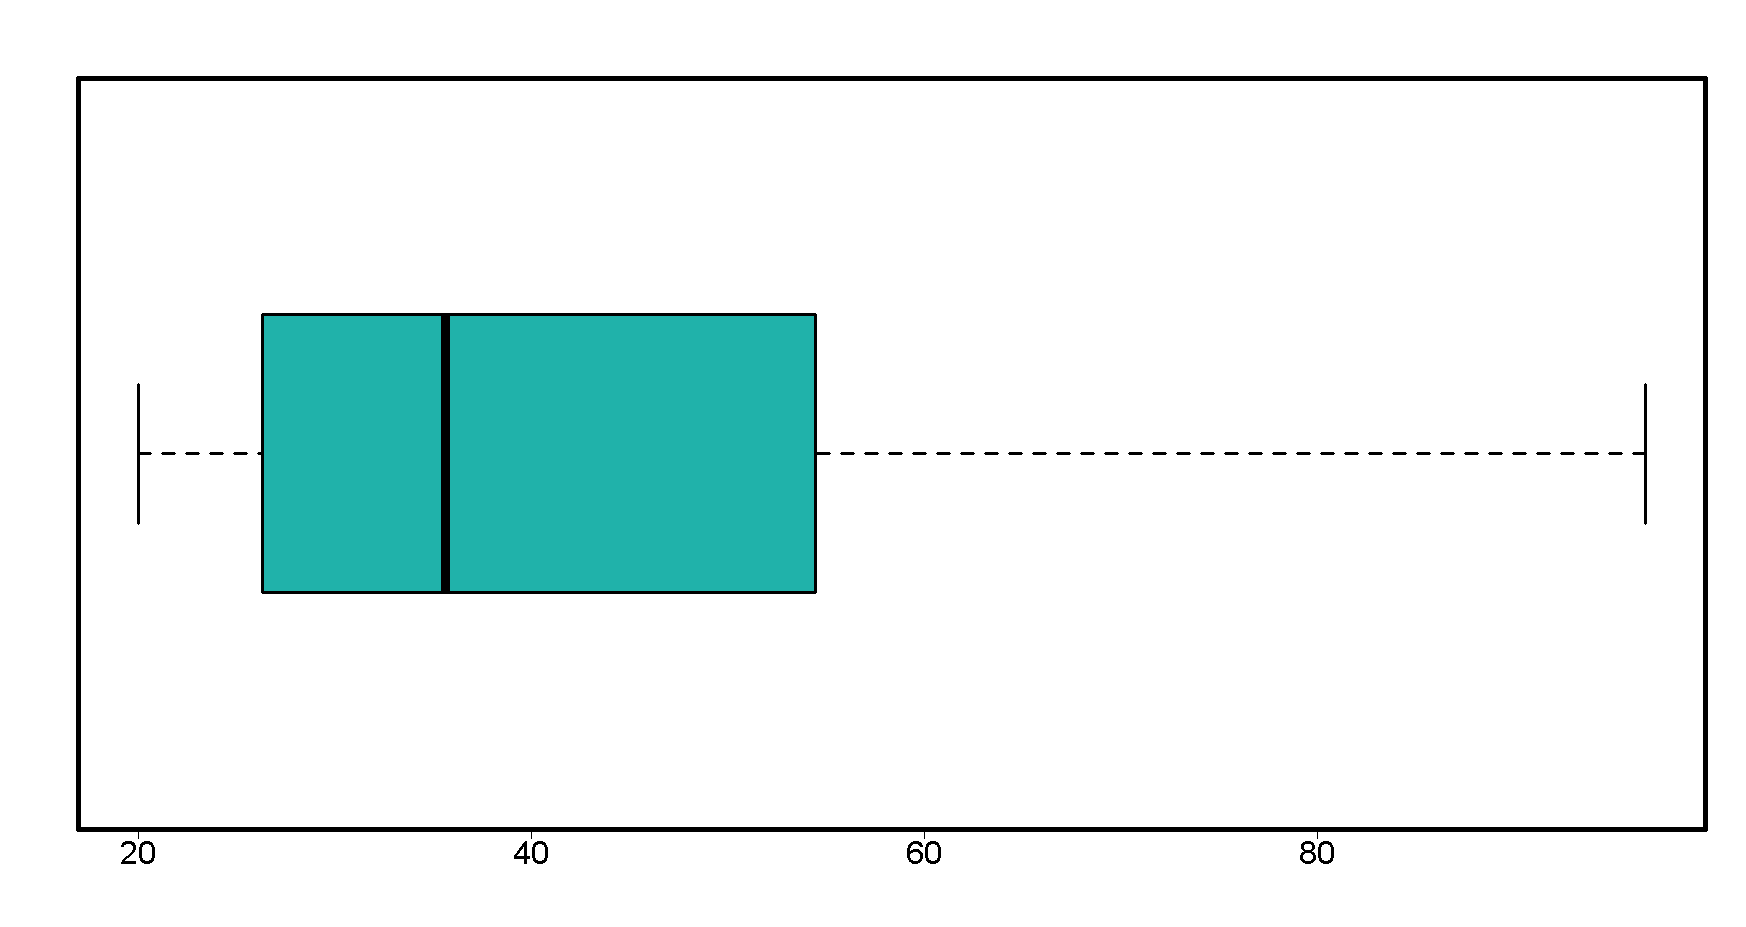
\includegraphics[width=16cm]{./datos/Tut12-CrateresBoxplotSinAtipicos.png}
% \end{center}
\caption{Boxplot, ahora sin los  valores atípicos, de la variable {\tt Diam\_km} del fichero {\tt Cap09-LolaLargeLunarCraterCatalog.csv}.}
\label{tut10:fig:BoxplotCrateres02}
\end{figure}

Ahora que hemos hecho la exploración inicial de la variable {\tt craterSize} podemos pensar cuál es la mejor forma de agruparla en clases. Cuando se agrupan los datos, hay dos alternativas básicas: usar intervalos de la misma anchura, o dividirlos en intervalos que tengan algún sentido en el contexto del problema.  En este caso, a la vista de los diagramas anteriores, hemos optado por dividirla en los siguientes cuatro intervalos (en km):
\[
[20,40], (40,60], (60,80], [80, )
\]
donde el último intervalo agrupa a todos los cráteres con un radio superior a 80km (y por tanto, a todos los atípicos de la Figura \ref{tut10:fig:BoxplotCrateres01}).

\begin{knitrout}
\definecolor{shadecolor}{rgb}{0.969, 0.969, 0.969}\color{fgcolor}\begin{kframe}
\begin{alltt}
\hlstd{craterSize} \hlkwb{=} \hlkwd{cut}\hlstd{(crateres}\hlopt{$}\hlstd{Diam_km,}
                 \hlkwc{breaks}\hlstd{=}\hlkwd{c}\hlstd{(}\hlkwd{seq}\hlstd{(}\hlnum{20}\hlstd{,} \hlnum{80}\hlstd{,} \hlnum{20}\hlstd{),} \hlkwd{max}\hlstd{(crateres}\hlopt{$}\hlstd{Diam_km)),}
                 \hlkwc{include.lowest}\hlstd{=}\hlnum{TRUE}\hlstd{)}
\end{alltt}
\end{kframe}
\end{knitrout}

El factor {\tt craterSize} resultante tiene esta tabla de frecuencias:
\begin{knitrout}
\definecolor{shadecolor}{rgb}{0.969, 0.969, 0.969}\color{fgcolor}\begin{kframe}
\begin{alltt}
\hlkwd{table}\hlstd{(craterSize)}
\end{alltt}
\begin{verbatim}
## craterSize
##       [20,40]       (40,60]       (60,80] (80,2.05e+03] 
##          3003          1108           482           592
\end{verbatim}
\end{kframe}
\end{knitrout}

Recuerda que la pregunta a la que estamos tratando de responder es si existe alguna relación entre el tamaño de los cráteres y su posición en uno u otro hemisferio. Es decir, usando los factores que acabamos de construir, si existe alguna relación entre {\tt hemisphere} y {\tt craterSize}. Para responder a la pregunta vamos a formularla como un contraste $\chi^2$ de independencia entre estos dos factores. La hipótesis nula de ese contraste sería:
\[H_0=\{\mbox{{\tt craterSize} es independiente de {\tt hemisphere}}\}.\]

% Estamos transformando variables cuantitativas continuas en factores. Recuerda que para hacer esta transformación, debemos agrupar los valores de estas variables en intervalos (clases), como vimos en la Sección \ref{curso-cap01:subsec:NotacionVariablesTablasFrecuenciaDatosAgrupados} del Capítulo \ref{curso-cap:IntroduccionEstadisticaDescriptiva} del libro. Cuando se agrupan los datos, hay dos alternativas: usar intervalos de la misma anchura, o dividirlos en intervalos que tengan algún sentido en el contexto del problema. En este caso, para obtener el factor {\tt hemisphere}, la variable {\tt lat} (latitud) se ha dividido en dos intervalos,
% \[(-90,0], (0,90]\]
% que indican simplemente si el cráter se encuentra situado en el hemisferio norte o en el sur.

% Vamos a estudiar la posible independencia de los factores {\tt hemisphere} y {\tt craterSize} mediante un contraste $\chi^2$.

Usaremos este ejemplo para ilustrar cómo podría ser un fichero de datos en bruto para este tipo de problemas y también veremos qué significa que los datos sean limpios en este contexto. Para empezar, vamos a trabajar con el fichero
\begin{center}
\fichero{../datos/Tut12-CrateresLunaEnBruto-01.csv}{Tut12-CrateresLunaEnBruto-01.csv}
\end{center}
Para ilustrar el contenido de ese fichero, aquí tienes sus primeras 10 filas (el fichero tiene más de 5000 filas de datos).


\begin{knitrout}
\definecolor{shadecolor}{rgb}{0.969, 0.969, 0.969}\color{fgcolor}\begin{kframe}
\begin{verbatim}
##    SUR NORTE X.20.40. X.40.60. X.60.80. X.80
## 1    1     0        0        0        1    0
## 2    1     0        1        0        0    0
## 3    0     1        0        0        1    0
## 4    0     1        1        0        0    0
## 5    0     1        0        1        0    0
## 6    1     0        0        1        0    0
## 7    1     0        0        0        0    1
## 8    1     0        1        0        0    0
## 9    1     0        0        1        0    0
## 10   1     0        1        0        0    0
\end{verbatim}
\end{kframe}
\end{knitrout}

Los datos que aparecen en este fichero corresponden a los niveles de los factores {\tt hemisphere} y {\tt craterSize}. Un $1$ en una columna significa que la observación corresponde a ese nivel del factor (y  un $0$ que no corresponde). Hemos elegido este formato para el fichero porque:
\begin{itemize}
  \item Este tipo de representación de los datos se encuentra a veces (especialmente en encuestas), cuando la persona que recoge los datos tiene un formulario con los campos predefinidos, con casillas correspondientes a las distintas clases, y tiene que marcar una de esas casillas (como sucede con los formularios OMR para lectoras ópticas, ver
\begin{center}
  \link{http://en.wikipedia.org/wiki/Optical_mark_recognition}{http://en.wikipedia.org/wiki/Optical\_mark\_recognition})
\end{center}
      Como puedes ver, en cada línea del fichero se describe un cráter. Las dos primeras columnas se han usado para indicar el hemisferio en el que se encuentra, mientras que las cuatro últimas indican a cuál de los cuatro niveles del factor {\tt craterSize} pertenece ese cráter.
  \item Por esa misma razón, no son datos limpios. Aunque cada fila corresponde a una observación individual, no se cumple que cada columna corresponda una variable.
    \item Además, entre ambos ficheros, se cubren las formas habituales de recoger los {\em datos de campo.} Date cuenta de que el diseño de la encuesta condiciona el formato en el que recibirás los datos y, por tanto,  el esfuerzo que habrá que dedicar a esquilarlos. Este proceso de recogida y formateo de los datos es también parte del Diseño Experimental. Una parte del trabajo que a menudo se obvia en las discusiones teóricas, pero que es esencial porque condiciona todo lo que podemos hacer después con los datos. En particular, fíjate en que puedes pasar del fichero {\tt Cap09-LolaLargeLunarCraterCatalog.csv} al {\tt Tut12-CrateresLunaEnBruto-01.csv}, pero no al revés porque al agrupar los datos se ha producido pérdida de información. Por eso es esencial tener claros los objetivos que perseguimos, para no desperdiciar recursos en conseguir datos innecesarios, a la vez que conservamos con mucho cuidado la información que, de hecho, hemos obtenido.

\end{itemize}

Aunque hemos fabricado este ejemplo con el propósito de ilustrar la discusión de esta Sección, puedes encontrar muchos otros, empezando por los que se incluyen en el artículo de H. Wickham citado en el Tutorial11.  El ejemplo resulta algo artificial porque disponiendo de los datos sin agrupar, lo razonable es obtener un fichero limpio de datos agrupados. Pero le pedimos indulgencia al lector; en el mundo real, en el que a menudo tenemos que trabajar con datos recogidos por otras personas, o por nosotros mismos si no hemos sido suficientemente cuidadosos, abundan los casos con ficheros como éste.

Usando la terminología de ese Tutorial11, ¿cómo podemos {\em esquilar} el fichero de datos para conseguir lo que queremos? En un ejemplo como este es relativamente sencillo, porque lo único que tenemos que hacer es {\em fusionar\,} todas las columnas que corresponden a una misma variable. En concreto, queremos pasar de esto:
\begin{knitrout}
\definecolor{shadecolor}{rgb}{0.969, 0.969, 0.969}\color{fgcolor}\begin{kframe}
\begin{alltt}
\hlstr{"SUR"},\hlstr{"NORTE"},\hlstr{"[20,40]"},\hlstr{"(40,60]"},\hlstr{"(60,80]"},\hlstr{">80"}
1,0,0,0,1,0
0,1,1,0,0,0
\end{alltt}
\end{kframe}
\end{knitrout}
a esto (la primera línea es la cabecera de los datos limpios):
\begin{knitrout}
\definecolor{shadecolor}{rgb}{0.969, 0.969, 0.969}\color{fgcolor}\begin{kframe}
\begin{alltt}
\hlstr{"hemisphere"}, \hlstr{"craterSize"}
\hlstr{"SUR"}, \hlstr{"(60,80]"}
\hlstr{"NORTE"}, \hlstr{"[20,40]"}
\end{alltt}
\end{kframe}
\end{knitrout}
Vamos a ver en detalle cómo hacer esto. Pero sería muy bueno que antes de ver la solución te tomes unos minutos para pensar cómo lo harías tú.

Una vez fijado el directorio de trabajo, leemos el fichero {\tt Tut12-CrateresLunaEnBruto-01.csv} en un {\tt data.frame} llamado {\tt crateresBruto}. Hemos renombrado las variables columna, porque no nos gustaban los nombres que R asigna automáticamente a las últimas cuatro columnas (otra posibilidad es usar la opción {\tt check.names} de la función {\tt read.tables}):

{\small
\begin{knitrout}
\definecolor{shadecolor}{rgb}{0.969, 0.969, 0.969}\color{fgcolor}\begin{kframe}
\begin{alltt}
\hlstd{crateresBruto} \hlkwb{=} \hlkwd{read.table}\hlstd{(}\hlkwc{file}\hlstd{=}\hlstr{"../datos/Tut12-CrateresLunaEnBruto-01.csv"}\hlstd{,}\hlkwc{header}\hlstd{=}\hlnum{TRUE}\hlstd{,}\hlkwc{sep}\hlstd{=}\hlstr{","}\hlstd{)}
\hlkwd{colnames}\hlstd{(crateresBruto)} \hlkwb{=} \hlkwd{c}\hlstd{(}\hlstr{"S"}\hlstd{,} \hlstr{"N"}\hlstd{,} \hlstr{"[20,40]"}\hlstd{,} \hlstr{"(40,60]"}\hlstd{,} \hlstr{"(60,80]"}\hlstd{,} \hlstr{"[80, )"}\hlstd{)}
\end{alltt}
\end{kframe}
\end{knitrout}
}

Ahora, fusionamos las dos primeras columnas en el vector {\tt hemisphere} así:

\begin{knitrout}
\definecolor{shadecolor}{rgb}{0.969, 0.969, 0.969}\color{fgcolor}\begin{kframe}
\begin{alltt}
\hlstd{hemisphere} \hlkwb{=} \hlkwd{ifelse}\hlstd{(crateresBruto[ ,}\hlnum{1}\hlstd{],} \hlkwc{yes} \hlstd{=} \hlstr{"SUR"}\hlstd{,} \hlkwc{no} \hlstd{=} \hlstr{"NORTE"}\hlstd{)}
\hlkwd{head}\hlstd{(hemisphere)}
\end{alltt}
\begin{verbatim}
## [1] "SUR"   "SUR"   "NORTE" "NORTE" "NORTE" "SUR"
\end{verbatim}
\end{kframe}
\end{knitrout}

Algunos comentarios sobre  este código:
\begin{itemize}
  \item Nos hemos aprovechado del hecho de que la información de las dos primeras columnas es redundante (si una es $1$, la otra es $0$ y viceversa) para trabajar sólo con la primera columna.
  \item Hemos usado la función {\tt ifelse} de R, que evalúa una condición lógica y devuelve el valor del argumento {\tt yes} cuando esa condición es cierta (en este ejemplo, devuelve la cadena de texto \verb#"SUR"#), pero si es falsa  devuelve el valor del argumento {\tt no} (en este ejemplo, devuelve la cadena de texto \verb#"NORTE"#). Además, hemos aprovechado el hecho de que R interpreta el número $1$ como {\tt TRUE}, y el número $0$ como {\tt FALSE}, directamente. Si quieres una versión más clara de lo que hemos hecho (sin esas conversiones implícitas de números en valores booleanos {\tt TRUE/FALSE}), puedes emplear esta línea de código alternativa:
\begin{knitrout}
\definecolor{shadecolor}{rgb}{0.969, 0.969, 0.969}\color{fgcolor}\begin{kframe}
\begin{alltt}
       \hlstd{hemisphere} \hlkwb{=} \hlkwd{ifelse}\hlstd{( crateresBruto[,}\hlnum{1}\hlstd{]} \hlopt{==} \hlnum{1}\hlstd{,} \hlkwc{yes} \hlstd{=} \hlstr{"SUR"}\hlstd{,} \hlkwc{no} \hlstd{=} \hlstr{"NORTE"}\hlstd{)}
\end{alltt}
\end{kframe}
\end{knitrout}
en la que explícitamente preguntamos si el valor de la primera columna es $1$.
\end{itemize}

Puedes comprobar que la tabla de frecuencias es la que hemos mostrado antes:
\begin{knitrout}
\definecolor{shadecolor}{rgb}{0.969, 0.969, 0.969}\color{fgcolor}\begin{kframe}
\begin{alltt}
\hlkwd{table}\hlstd{(hemisphere)}
\end{alltt}
\begin{verbatim}
## hemisphere
## NORTE   SUR 
##  2402  2783
\end{verbatim}
\end{kframe}
\end{knitrout}
¿Te has fijado en el orden en que aparecen las variables en esta tabla? ¿De qué tipo es la variable {\tt hemisphere}?

\begin{ejercicio}
\label{tut12:ejercicio04}
Responde a esa pregunta. Queremos que la variable {\tt hemisphere} sea un factor. Así que si no lo es, conviértela en un factor. Soluciones en la página \pageref{tut12:ejercicio04:sol}.
\qed
\end{ejercicio}

La idea que vamos a usar para fusionar las cuatro últimas columnas en un vector {\tt craterSize} es similar. Pero ahora, puesto que tenemos que inspeccionar las cuatro últimas columnas (de la tercera a la sexta) ya no hay la misma redundancia en los datos de la que nos podamos aprovechar. La primera idea que se te puede ocurrir es usar un bucle {\tt for} para recorrer las filas de la matriz y, para cada una ellas, usar la función {\tt which} para localizar cuál es igual a $1$. Enseguida verás por qué le hemos puesto el nombre {\tt primerIntento} al resultado:

\begin{knitrout}
\definecolor{shadecolor}{rgb}{0.969, 0.969, 0.969}\color{fgcolor}\begin{kframe}
\begin{alltt}
\hlstd{primerIntento} \hlkwb{=} \hlkwd{c}\hlstd{()}
\hlkwa{for}\hlstd{(i} \hlkwa{in} \hlnum{1}\hlopt{:}\hlkwd{nrow}\hlstd{(crateresBruto))\{}
  \hlstd{datosCrater} \hlkwb{=} \hlstd{crateresBruto[i,} \hlnum{3}\hlopt{:}\hlnum{6}\hlstd{]}
  \hlstd{craterSizeTipo} \hlkwb{=} \hlkwd{which}\hlstd{(datosCrater} \hlopt{==} \hlnum{1}\hlstd{)}
  \hlstd{primerIntento} \hlkwb{=} \hlkwd{c}\hlstd{(primerIntento, craterSizeTipo)}
\hlstd{\}}
\end{alltt}
\end{kframe}
\end{knitrout}

Queremos aprovechar este ejemplo para inivitar al lector a reflexionar sobre la eficiencia del código en R. Hasta este punto, en los distintos tutoriales nos hemos limitado a resolver los problemas sin preocuparnos demasiado de esto. Eso es justificable cuando está aprendiendo y mientras los problemas son de un tamaño modesto, como los que hemos ido encontrando en este curso. Pero al enfrentarnos a problemas del mundo real, se hace cada vez más necesario preocuparnos de que nuestro código sea {\em eficiente}. En este sentido, en el anterior fragmento de código hemos hecho las cosas casi de la peor manera posible. En R es {\bf esencial usar operaciones vectorializadas y evitar los bucles} ({\tt for, while, repeat}) siempre que sea posible.

Para ver un ejemplo inicial sencillo de esto vamos a usar una herramienta que R pone a nuestra disposición para medir el tiempo de ejecución de un fragmento de código: la función {\tt system.time}. Esta función se puede usar para obtener una medida objetiva de ese tiempo de ejecución. Para usarla, basta con incluir como argumento el fragmento de dódigo cuya eficiencia queremos analizar. Por ejemplo, vamos a generar un vector de $10000000$ números aleatorios y luego vamos a sumarle $1$ a cada uno de esos números. Pero vamos a hacerlo de dos maneras distintas. En la primera versión usaremos un bucle {\tt for} para acceder uno a uno a los elementos del vector. En la segunda, la versión vectorializada, simplemente usamos la aritmética vectorial de R.
\begin{knitrout}
\definecolor{shadecolor}{rgb}{0.969, 0.969, 0.969}\color{fgcolor}\begin{kframe}
\begin{alltt}
\hlstd{n} \hlkwb{=} \hlnum{10000000}
\hlstd{v} \hlkwb{=} \hlkwd{rnorm}\hlstd{(n)}
\hlkwd{system.time}\hlstd{(}
  \hlkwa{for} \hlstd{(i} \hlkwa{in} \hlnum{1}\hlopt{:}\hlstd{n)\{}
    \hlstd{v[i]} \hlkwb{=} \hlstd{v[i]} \hlopt{+} \hlnum{1}
  \hlstd{\}}
\hlstd{)}
\end{alltt}
\begin{verbatim}
##    user  system elapsed 
##   18.59    0.05   19.22
\end{verbatim}
\begin{alltt}
\hlkwd{system.time}\hlstd{(v} \hlkwb{<-} \hlstd{v} \hlopt{+}\hlnum{1}\hlstd{)}
\end{alltt}
\begin{verbatim}
##    user  system elapsed 
##    0.01    0.00    0.02
\end{verbatim}
\end{kframe}
\end{knitrout}
El tiempo que aparece en la respuesta se mide en segundos. Como puedes ver, la segunda versión es varios órdenes de magnitud más rápida que la primera.

Volviendo a la fusión de columnas en el fichero ¿ccómo podemos hacerlo de manera eficiente? Usando una operación vectorializada, en este caso mediante la familia de funciones {\tt apply} (que incluye {\tt apply}, pero también {\tt mapply, sapply, lapply,...}). Para hacer eso defininos una función, a la que hemos llamado {\tt claseCrater}, que codifica la operación que queremos hacer en cada fila de la tabla de datos:
\begin{knitrout}
\definecolor{shadecolor}{rgb}{0.969, 0.969, 0.969}\color{fgcolor}\begin{kframe}
\begin{alltt}
\hlstd{claseCrater} \hlkwb{=} \hlkwa{function}\hlstd{(}\hlkwc{datosCrater}\hlstd{)\{}
  \hlstd{craterSize} \hlkwb{=} \hlkwd{which}\hlstd{(datosCrater} \hlopt{==} \hlnum{1}\hlstd{)}
\hlstd{\}}
\end{alltt}
\end{kframe}
\end{knitrout}

Una vez hecho esto, usamos {\tt apply} para aplicar esta función al fragmento de {\tt crateresBruto} que contiene la información sobre la clase del tamaño del crater. El argumento {\tt MARGIN} sirve para indicarle a R que queremos trabajar {\em por filas}:
\begin{knitrout}
\definecolor{shadecolor}{rgb}{0.969, 0.969, 0.969}\color{fgcolor}\begin{kframe}
\begin{alltt}
\hlstd{craterSize} \hlkwb{=} \hlkwd{apply}\hlstd{(crateresBruto[,} \hlnum{3}\hlopt{:}\hlnum{6}\hlstd{],} \hlkwc{MARGIN} \hlstd{=} \hlnum{1}\hlstd{,} \hlkwc{FUN} \hlstd{= claseCrater)}
\end{alltt}
\end{kframe}
\end{knitrout}
El resultado es un vector con el mismo número de elementos que filas hay en la tabla y que contiene, en cada posición, el resultado de aplicar  {\tt claseCrater} a la correspondiente fila de la tabla. Podemos empezar por comprobar que el resultado de nuestro primer intento coincide con el de {\tt apply}:
\begin{knitrout}
\definecolor{shadecolor}{rgb}{0.969, 0.969, 0.969}\color{fgcolor}\begin{kframe}
\begin{alltt}
\hlkwd{table}\hlstd{(craterSize} \hlopt{-} \hlstd{primerIntento)}
\end{alltt}
\begin{verbatim}
## 
##    0 
## 5185
\end{verbatim}
\end{kframe}
\end{knitrout}
Así que tenemos dos formas de resolver el mismo problema. ¿Cuál es mejor? Hay varios sentidos en los que podemos medir esto: la rapidez es uno de ellos, desde luego. Pero también podemos preocuparnos por la sencillez del código. En ese sentido, la solución con {\tt apply} es más abstracta, pero precisamente por eso resulta más simple (cabe en dos líneas de código). Al principio te costará valorarlo, pero a medida que ganes experiencia programando con R empezarás a apreciar la ventaja que supone ese nivel de abstracción. Y, en cualquier caso, volviendo al asunto de la velocidad, dependiendo de la potencia del ordenador que estés usando  es posible que  hayas podido percibir directamente la diferencia entre ambos métodos. Para obtener una medida más objetiva podemos usar una herramienta que R pone a nuestra disposición para medir el tiempo de ejecución de un fragmento de código: la función {\tt }. Esta función se puede usar para incluir como argumento el fragmento de dódigo cuya eficiencia queremos analizar. Por ejemplo, para nuestro primer intento es:

\begin{knitrout}
\definecolor{shadecolor}{rgb}{0.969, 0.969, 0.969}\color{fgcolor}\begin{kframe}
\begin{alltt}
\hlkwd{set.seed}\hlstd{(}\hlnum{2015}\hlstd{)}
\hlkwd{system.time}\hlstd{(\{}
  \hlstd{primerIntento} \hlkwb{=} \hlkwd{c}\hlstd{()}
  \hlkwa{for}\hlstd{(i} \hlkwa{in} \hlnum{1}\hlopt{:}\hlkwd{nrow}\hlstd{(crateresBruto))\{}
    \hlstd{datosCrater} \hlkwb{=} \hlstd{crateresBruto[i,} \hlnum{3}\hlopt{:}\hlnum{6}\hlstd{]}
    \hlstd{craterSizeTipo} \hlkwb{=} \hlkwd{which}\hlstd{(datosCrater} \hlopt{==} \hlnum{1}\hlstd{)}
    \hlstd{primerIntento} \hlkwb{=} \hlkwd{c}\hlstd{(primerIntento, craterSizeTipo)}
  \hlstd{\}}
\hlstd{\})}
\end{alltt}
\begin{verbatim}
##    user  system elapsed 
##    0.92    0.00    0.92
\end{verbatim}
\end{kframe}
\end{knitrout}
El dato más útil aquí es {\tt elpased}, el tiempo en segundos que hemos empleado (hay muchos detalles técnicos en juego en la interpreteación de estos valores, pero para un caso sencillo basta con comparar {\tt elapsed})

Mientras que para el segundo es:
\begin{knitrout}
\definecolor{shadecolor}{rgb}{0.969, 0.969, 0.969}\color{fgcolor}\begin{kframe}
\begin{alltt}
\hlkwd{system.time}\hlstd{(\{}
  \hlstd{claseCrater} \hlkwb{=} \hlkwa{function}\hlstd{(}\hlkwc{datosCrater}\hlstd{)\{}
    \hlstd{craterSize} \hlkwb{=} \hlkwd{which}\hlstd{(datosCrater} \hlopt{==} \hlnum{1}\hlstd{)}
  \hlstd{\}}
\hlstd{craterSize} \hlkwb{=} \hlkwd{apply}\hlstd{(crateresBruto[,} \hlnum{3}\hlopt{:}\hlnum{6}\hlstd{],} \hlkwc{MARGIN} \hlstd{=} \hlnum{1}\hlstd{,} \hlkwc{FUN} \hlstd{= claseCrater)}
\hlstd{\})}
\end{alltt}
\begin{verbatim}
##    user  system elapsed 
##    0.03    0.00    0.03
\end{verbatim}
\end{kframe}
\end{knitrout}
La diferencia no es tan espectacular como antes, pero aún así es muy grande, de órdenes de magnitud. Confiamos en que este simple ejemplo haya estimulado tu curiosidad y te sirva como motivación para tratar de profundizar en el tema de la eficiencia en programación.

Volviendo a nuestro problema, la tabla de frecuencias de {\tt craterSize} es la esperada:
\begin{knitrout}
\definecolor{shadecolor}{rgb}{0.969, 0.969, 0.969}\color{fgcolor}\begin{kframe}
\begin{alltt}
\hlkwd{table}\hlstd{(craterSize)}
\end{alltt}
\begin{verbatim}
## craterSize
##    1    2    3    4 
## 3003 1108  482  592
\end{verbatim}
\end{kframe}
\end{knitrout}

Un detalle: tal como lo hemos construido, el vector {\tt craterSize} no es un factor.

\begin{knitrout}
\definecolor{shadecolor}{rgb}{0.969, 0.969, 0.969}\color{fgcolor}\begin{kframe}
\begin{alltt}
\hlkwd{class}\hlstd{(craterSize)}
\end{alltt}
\begin{verbatim}
## [1] "integer"
\end{verbatim}
\end{kframe}
\end{knitrout}
Pero podemos convertirlo fácilmente en un factor:
\begin{knitrout}
\definecolor{shadecolor}{rgb}{0.969, 0.969, 0.969}\color{fgcolor}\begin{kframe}
\begin{alltt}
\hlstd{craterSize} \hlkwb{=} \hlkwd{factor}\hlstd{(craterSize,}
                \hlkwc{labels} \hlstd{=} \hlkwd{c}\hlstd{(}\hlstr{"[20,40]"}\hlstd{,} \hlstr{"(40,60]"}\hlstd{,} \hlstr{"(60,80]"}\hlstd{,} \hlstr{"[80, )"}\hlstd{))}
\end{alltt}
\end{kframe}
\end{knitrout}
Ahora que ya tenemos los dos vectores, con los niveles de ambos factores, obtener la tabla de contingencia (son sus valores marginales), y el contraste $\chi^2$ de homogeneidad es muy fácil. Basta con usar:

\begin{knitrout}
\definecolor{shadecolor}{rgb}{0.969, 0.969, 0.969}\color{fgcolor}\begin{kframe}
\begin{alltt}
\hlkwd{addmargins}\hlstd{(}\hlkwd{table}\hlstd{(hemisphere, craterSize))}
\end{alltt}
\begin{verbatim}
##           craterSize
## hemisphere [20,40] (40,60] (60,80] [80, )  Sum
##      NORTE    1388     523     227    264 2402
##      SUR      1615     585     255    328 2783
##      Sum      3003    1108     482    592 5185
\end{verbatim}
\begin{alltt}
\hlkwd{chisq.test}\hlstd{(hemisphere, craterSize)}
\end{alltt}
\begin{verbatim}
## 
## 	Pearson's Chi-squared test
## 
## data:  hemisphere and craterSize
## X-squared = 1.18, df = 3, p-value = 0.76
\end{verbatim}
\end{kframe}
\end{knitrout}

\begin{ejercicio}
\label{tut12:ejercicio05}
¿Cuál es la hipótesis nula, y cuál la conclusión del contraste que acabamos de pedirle a R que haga?
%Soluciones en la página \pageref{tut12:ejercicio05:sol}.
\qed
\end{ejercicio}


Ahora  podemos ver más claramente lo que significa la idea de {\em datos limpios} para un contraste $\chi^2$  como este. Si usamos los vectores {\tt hemisphere} y {\tt craterSize} para crear un {\tt data.frame} llamado {\tt craterDatosLimpios}, de esta manera:
\begin{knitrout}
\definecolor{shadecolor}{rgb}{0.969, 0.969, 0.969}\color{fgcolor}\begin{kframe}
\begin{alltt}
\hlstd{craterDatosLimpios} \hlkwb{=} \hlkwd{data.frame}\hlstd{(hemisphere, craterSize)}
\end{alltt}
\end{kframe}
\end{knitrout}
entonces las primeras filas de este {\tt data.frame} son:
\begin{knitrout}
\definecolor{shadecolor}{rgb}{0.969, 0.969, 0.969}\color{fgcolor}\begin{kframe}
\begin{alltt}
\hlkwd{head}\hlstd{(craterDatosLimpios,}\hlnum{10}\hlstd{)}
\end{alltt}
\begin{verbatim}
##    hemisphere craterSize
## 1         SUR    (60,80]
## 2         SUR    [20,40]
## 3       NORTE    (60,80]
## 4       NORTE    [20,40]
## 5       NORTE    (40,60]
## 6         SUR    (40,60]
## 7         SUR     [80, )
## 8         SUR    [20,40]
## 9         SUR    (40,60]
## 10        SUR    [20,40]
\end{verbatim}
\end{kframe}
\end{knitrout}
Y confirman que estamos ante una estructura de datos limpia, en el sentido que venimos utilizando:
\begin{itemize}
  \item Una fila para cada observación individual.
  \item Una columna para cada variable.
\end{itemize}
Si ahora queremos guardar estos datos limpios en un fichero {\tt csv}, basta con usar:
y obtendremos el fichero que queríamos.
\begin{knitrout}
\definecolor{shadecolor}{rgb}{0.969, 0.969, 0.969}\color{fgcolor}\begin{kframe}
\begin{alltt}
\hlkwd{write.table}\hlstd{(craterDatosLimpios,} \hlkwc{file}\hlstd{=}\hlstr{"../datos/Tut12-CrateresLunaEnBruto.csv"}\hlstd{,}
    \hlkwc{sep}\hlstd{=}\hlstr{","}\hlstd{,} \hlkwc{row.names}\hlstd{=}\hlnum{FALSE}\hlstd{,} \hlkwc{col.names}\hlstd{=}\hlnum{TRUE}\hlstd{)}
\end{alltt}
\end{kframe}
\end{knitrout}


\section{Contrastes  $\chi^2$ en otros programas.}
\label{tut12:sec:ContrasteChiCuadradoOtrosProgramas}

\subsection{GeoGebra.}

En GeoGebra es muy fácil hacer contrastes $\chi^2$ de independencia usando la {\em Calculadora de Probabilidades} (pestaña {\em Estadísticas}). Por ejemplo, en la siguiente figura tienes el resultado que se obtiene para los datos del Ejemplo del {\em Barómetro del CIS}.

\begin{center}
    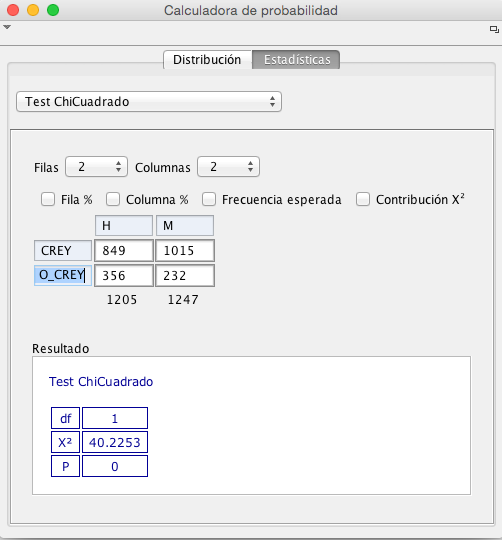
\includegraphics[height=8cm]{../fig/Tut12-GeoGebraChiCuadradoIndependencia.png}
\end{center}


\begin{ejercicio}
\label{tut12:ejercicio05}
Usa GeoGebra para comprobar los resultados del Ejemplo \ref{curso-cap12:ejem:Avutardas} del libro (pág. \pageref{curso-cap12:ejem:Avutardas}), el de las poblaciones de Avutardas.
%Soluciones en la página \pageref{tut12:ejercicio05:sol}.
\qed
\end{ejercicio}

Y también es posible obtener un contraste de homogeneidad, como hemos hecho en la siguiente figura para el Ejemplo \ref{curso-cap12:ejem:Mendel} del libro (pág. \pageref{curso-cap12:ejem:Mendel}), el de Mendel y sus guisantes.
\begin{center}
    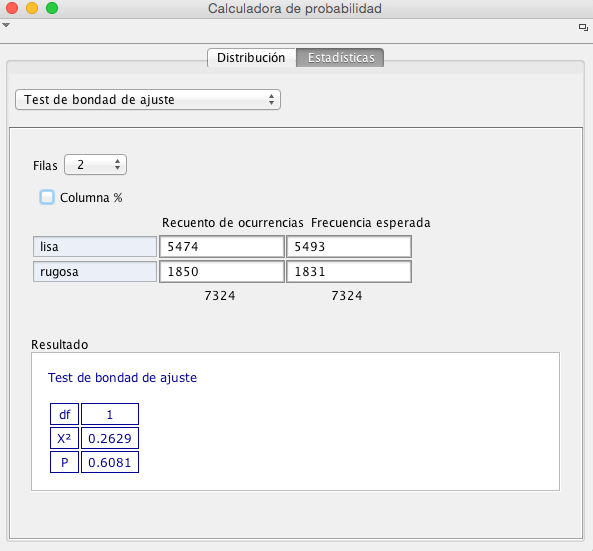
\includegraphics[height=8cm]{../fig/Tut12-GeoGebraChiCuadradoHomogeneidad.png}
\end{center}

Si en alguna ocasión necesitas o prefieres usar la {\em Línea de Entrada} o la vista {\em CAS}, GeoGebra pone a nuestra disposición la función {\tt TestChiCuadrado}, con la que podemos hacer todos estos contrastes. No dejes de consultar la ayuda de esa función antes de utilizarla.

\subsection{Calc.}

Queremos comentar, muy brevemente, las posibilidades que ofrece la hoja de cálculo Calc para este tipo de contrastes. Aunque a estas alturas del curso esperamos haber persuadido al lector de las ventajas de un software especializado (como R), en alguna ocasión puede ser necesario utilizar esta herramienta básica.

Calc nos ofrece la función {\tt PRUEBA.CHI} ({\tt CHITEST}, en la versión en inglés de Calc) para este tipo de contrastes. En la Figura \ref{tut10:fig:Calc01} puedes ver como la usamos para el Ejemplo \ref{curso-cap12:ejem:BarometroCIS01} del libro, el del {\em Barómetro} del CIS.

La función {\tt PRUEBA.CHI} usa dos tablas de valores, almacenadas en sendos rangos de celdas, para los valores observados y esperados. ¿Los grados de libertad? Se determinan a partir de las dimensiones (número de filas y columnas) de esas tablas (que desde luego, deben coincidir).  El resultado es el p-valor del contraste que, como puedes ver, coincide con el valor que hemos obtenido en R. Si se desea calcular el valor del estadístico del contraste, tenemos que hacerlo manualmente. Por ejemplo, en la celda {\tt A11} de la Figura \ref{tut10:fig:Calc01} nosotros hemos incluido el código:
\begin{verbatim}
=(A3-D3)^2/D3
\end{verbatim}
y hemos hecho lo propio en el rango {\tt A11:B12}. El estadístico se calcula después sumando los valores de ese rango de residuos estudentizados. El fichero adjunto
\begin{center}
\fichero{../ods/Tut12-BarometroCIS.ods}{Tut12-BarometroCIS.ods}
\end{center}
contiene esa hoja de cálculo, que con algunas modificaciones puede adaptarse a otros ejemplos.

\begin{figure}[t]
\begin{center}
    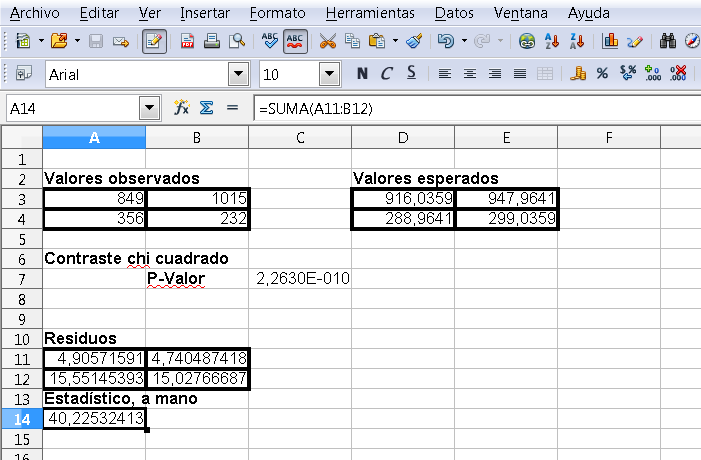
\includegraphics[height=8cm]{../fig/Tut12-Calc01.png}
\end{center}
\caption{La función {\tt PRUEBA.CHI} de Calc, para el contraste $\chi^2$ de independencia con los datos del Barómetro del CIS}
\label{tut10:fig:Calc01}
\end{figure}


¿Y si lo que queremos es hacer un contraste $\chi^2$ de homogeneidad? Usamos la misma función {\tt PRUEBA.CHI}.  Basta, en ese caso, con que los valores observados y esperados ocupen rangos unidimensionales (cada uno de ellos en una fila o una columna). Por ejemplo, en la Figura \ref{tut10:fig:Calc02} puedes ver esa función aplicada a los datos del Ejemplo \ref{curso-cap12:ejem:DadoCargado} del libro, el del dado cargado.


\begin{figure}[tb]
\begin{center}
    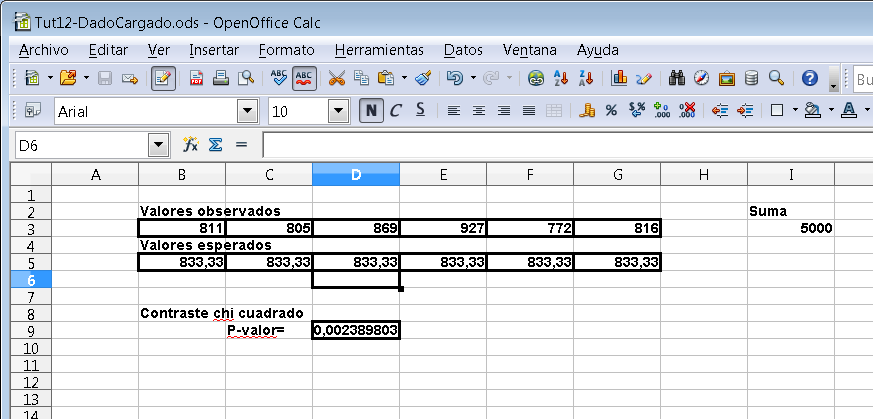
\includegraphics[height=6cm]{../fig/Tut12-Calc02.png}
\end{center}
\caption{La función {\tt PRUEBA.CHI} de Calc, para el contraste $\chi^2$ de homogeneidad con los datos del Ejemplo \ref{curso-cap12:ejem:DadoCargado} del libro.}
\label{tut10:fig:Calc02}
\end{figure}
De nuevo, si se desea el valor del estadístico, es necesario calcularlo {\em a mano}. El fichero de este ejemplo es:
\begin{center}
\fichero{../ods/Tut12-DadoCargado.ods}{Tut12-DadoCargado.ods}
\end{center}

\paragraph{Ejercicio:}\label{tut12:ejercicio07}\quad\\
Usa Calc para obtener el estadístico de este último ejemplo. Y calcula, también con Calc, los p-valores de los Ejemplos \ref{curso-cap12:ejem:Avutardas} (avutardas) y \ref{curso-cap12:ejem:Mendel} (Mendel) del libro.
\qed



\section{El contraste exacto de Fisher. Distribución hipergeométrica.}

Vamos a ver como utilizar R para obtener los resultados del Ejemplo \ref{curso-cap12:ejem:MetodoFisher01} del libro (pág. \pageref{curso-cap12:ejem:MetodoFisher01}) y de sus continuaciones en los ejemplos del \ref{curso-cap12:ejem:MetodoFisher02} hasta el  \ref{curso-cap12:ejem:MetodoFisher06} (pág. \pageref{curso-cap12:ejem:MetodoFisher06}), en el que finalmente hemos obtenido el p-valor del contraste. A estas alturas, el lector seguramente espera que R tenga funciones casi para cualquier cosa. Así que empecemos esta vez por lo más sencillo. Para obtener ese p-valor que aparece en el Ejemplo \ref{curso-cap12:ejem:MetodoFisher06} basta con aplicar la función {\tt fisher.test} a los datos de la tabla de contingencia observada:

{\small
\begin{knitrout}
\definecolor{shadecolor}{rgb}{0.969, 0.969, 0.969}\color{fgcolor}\begin{kframe}
\begin{alltt}
\hlstd{(fisherTest} \hlkwb{=} \hlkwd{fisher.test}\hlstd{(}\hlkwd{matrix}\hlstd{(}\hlkwd{c}\hlstd{(}\hlnum{9}\hlstd{,} \hlnum{6}\hlstd{,} \hlnum{3}\hlstd{,} \hlnum{12}\hlstd{),} \hlkwc{nrow} \hlstd{=} \hlnum{2}\hlstd{),} \hlkwc{alternative} \hlstd{=} \hlstr{"greater"}\hlstd{))}
\end{alltt}
\begin{verbatim}
## 
## 	Fisher's Exact Test for Count Data
## 
## data:  matrix(c(9, 6, 3, 12), nrow = 2)
## p-value = 0.03
## alternative hypothesis: true odds ratio is greater than 1
## 95 percent confidence interval:
##  1.1833    Inf
## sample estimates:
## odds ratio 
##     5.6137
\end{verbatim}
\end{kframe}
\end{knitrout}
}

Como ves, el p-valor coincide con el que hemos obtenido en el ejemplo del libro. Ahora queremos reconstruir paso a paso el cálculo manual de ese p-valor. Pero antes, dado que la vamos a necesitar, veamos brevemente como se trabaja en R con la distribución hipergeométrica.

\subsubsection*{La distribución hipergeométrica en R.}
\label{tut12:subsubsec:DistHipergeometricaR}

El lector no se sorprenderá si le decimos que R dispone del cuarteto habitual de funciones {\tt d, p, q, r}, en este caso identificadas por el sufijo {\tt hyper}. Recuerda que pensamos en una caja con $N$ bolas, de las cuales $B$ son blancas. Extraemos una muestra de $m$ bolas de la caja, {\bf sin reemplazamiento}, y nos preguntamos por la probabilidad de que $k$ de las bolas extraídas sean blancas.

Esta es la notación que hemos usado en el libro, porque creemos que aporta claridad. Desafortunadamente, en R las funciones relacionadas con la hipergeométrica usan una notación distinta y, hasta cierto punto, conflictiva con la que usamos nosotros. Por ejemplo, en la función
\begin{knitrout}
\definecolor{shadecolor}{rgb}{0.969, 0.969, 0.969}\color{fgcolor}\begin{kframe}
\begin{alltt}
\hlkwd{dhyper}\hlstd{(x, m, n, k)}
\end{alltt}
\end{kframe}
\end{knitrout}
la ayuda de R nos indica que:
\begin{itemize}
  \item {\tt m} representa el número de bolas blancas en la urna. Lo hemos llamado $B$ en el libro.
  \item {\tt n} representa el número de bolas negras en la urna.  En el libro no tiene un nombre asignado, es $N - B$.
  \item {\tt k} representa el número de bolas que se extraen de la caja. Aquí es donde hay más riesgo de confusión, porque nosotros lo hemos llamado $m$.
  \item {\tt x} es el número de bolas (blancas entre las extraídas) del que queremos calcular la probabilidad. Y que, para aumentar la confusión, nosotros llamamos $k$.
\end{itemize}
Para no perdernos en este embrollo de símbolos recomendamos encarecidamente el uso del tabulador en RStudio y mantener a la vista la Tabla \ref{curso-cap12:tabla:TraduccionFisherHipergeometrica} del libro (pág. \pageref{curso-cap12:tabla:TraduccionFisherHipergeometrica}). De esa forma, cuando uses R, podrás asegurarte de que asignas a cada parámetro el valor que realmente deseas.

Si, por ejemplo, trabajamos con una distribución hipergeométrica $Hyp(N=200, B=130, m=50)$, entonces la probabilidad de extraer exactamente $k=17$ bolas blancas es

\begin{knitrout}
\definecolor{shadecolor}{rgb}{0.969, 0.969, 0.969}\color{fgcolor}\begin{kframe}
\begin{alltt}
\hlkwd{dhyper}\hlstd{(}\hlkwc{x} \hlstd{=} \hlnum{17}\hlstd{,} \hlkwc{m} \hlstd{=} \hlnum{130}\hlstd{,} \hlkwc{n} \hlstd{=} \hlnum{200} \hlopt{-} \hlnum{130}\hlstd{,} \hlkwc{k} \hlstd{=} \hlnum{50}\hlstd{)}
\end{alltt}
\begin{verbatim}
## [1] 1.7995e-07
\end{verbatim}
\end{kframe}
\end{knitrout}
mientras que la probabilidad de obtener $17$ o menos es:

\begin{knitrout}
\definecolor{shadecolor}{rgb}{0.969, 0.969, 0.969}\color{fgcolor}\begin{kframe}
\begin{alltt}
\hlkwd{phyper}\hlstd{(}\hlkwc{q} \hlstd{=} \hlnum{17}\hlstd{,} \hlkwc{m} \hlstd{=} \hlnum{130}\hlstd{,} \hlkwc{n} \hlstd{=} \hlnum{200} \hlopt{-} \hlnum{130}\hlstd{,} \hlkwc{k} \hlstd{=} \hlnum{50}\hlstd{)}
\end{alltt}
\begin{verbatim}
## [1] 2.1392e-07
\end{verbatim}
\end{kframe}
\end{knitrout}

El cuantil $0.75$ de esa distribución hipergeométrica se obtiene con:

\begin{knitrout}
\definecolor{shadecolor}{rgb}{0.969, 0.969, 0.969}\color{fgcolor}\begin{kframe}
\begin{alltt}
\hlkwd{qhyper}\hlstd{(}\hlkwc{p} \hlstd{=} \hlnum{0.75}\hlstd{,} \hlkwc{m} \hlstd{=} \hlnum{130}\hlstd{,} \hlkwc{n} \hlstd{=} \hlnum{200} \hlopt{-} \hlnum{130}\hlstd{,} \hlkwc{k} \hlstd{=} \hlnum{50}\hlstd{)}
\end{alltt}
\begin{verbatim}
## [1] 34
\end{verbatim}
\end{kframe}
\end{knitrout}

\begin{ejercicio}
\label{tut12:ejercicio06}
Interpreta este resultado en términos de probabilidad.
%Soluciones en la página \pageref{tut12:ejercicio06:sol}.
\qed
\end{ejercicio}

Finalmente, si lo que queremos es obtener valores aleatorios de esa distribución, por ejemplo para simular varias extracciones de muestras del mismo tamaño de esa caja, usaremos {\tt rhyper}:

\begin{knitrout}
\definecolor{shadecolor}{rgb}{0.969, 0.969, 0.969}\color{fgcolor}\begin{kframe}
\begin{alltt}
\hlkwd{rhyper}\hlstd{(}\hlnum{20}\hlstd{,} \hlkwc{m} \hlstd{=} \hlnum{130}\hlstd{,} \hlkwc{n} \hlstd{=} \hlnum{200} \hlopt{-} \hlnum{130}\hlstd{,} \hlkwc{k} \hlstd{=} \hlnum{50}\hlstd{)}
\end{alltt}
\begin{verbatim}
##  [1] 34 36 32 31 30 35 29 30 35 38 32 30 33 31 36 34 32 31 30 33
\end{verbatim}
\end{kframe}
\end{knitrout}

El resultado indica el número de bolas blancas que contiene cada una de las $20$ muestras de $50$ bolas que hemos extraído.

\subsubsection*{El contraste de Fisher paso a paso.}

Volvamos al Ejemplo del libro. Empezamos con la tabla de valores observados, que aparece en el Ejemplo \ref{curso-cap12:ejem:MetodoFisher03} (pág. \pageref{curso-cap12:ejem:MetodoFisher03}), a la que le añadimos las decoraciones habituales:
\begin{knitrout}
\definecolor{shadecolor}{rgb}{0.969, 0.969, 0.969}\color{fgcolor}\begin{kframe}
\begin{alltt}
\hlstd{(tablaObservada} \hlkwb{=} \hlkwd{matrix}\hlstd{(} \hlkwd{c}\hlstd{(}\hlnum{9}\hlstd{,} \hlnum{3}\hlstd{,} \hlnum{6}\hlstd{,} \hlnum{12}\hlstd{),}  \hlkwc{nrow}\hlstd{=} \hlnum{2}\hlstd{,} \hlkwc{byrow} \hlstd{=} \hlnum{TRUE}\hlstd{))}
\end{alltt}
\begin{verbatim}
##      [,1] [,2]
## [1,]    9    3
## [2,]    6   12
\end{verbatim}
\begin{alltt}
\hlkwd{colnames}\hlstd{(tablaObservada)} \hlkwb{=} \hlkwd{c}\hlstd{(}\hlstr{"Expuestos"}\hlstd{,} \hlstr{"NoExpuestos"}\hlstd{)}
\hlkwd{rownames}\hlstd{(tablaObservada)} \hlkwb{=} \hlkwd{c}\hlstd{(}\hlstr{"Enfermos"}\hlstd{,} \hlstr{"Sanos"} \hlstd{)}
\hlkwd{addmargins}\hlstd{(tablaObservada)}
\end{alltt}
\begin{verbatim}
##          Expuestos NoExpuestos Sum
## Enfermos         9           3  12
## Sanos            6          12  18
## Sum             15          15  30
\end{verbatim}
\end{kframe}
\end{knitrout}
Llamemos a esta tabla {\tt tabla0}.
\begin{knitrout}
\definecolor{shadecolor}{rgb}{0.969, 0.969, 0.969}\color{fgcolor}\begin{kframe}
\begin{alltt}
\hlstd{tabla0} \hlkwb{=} \hlstd{tablaObservada}
\end{alltt}
\end{kframe}
\end{knitrout}

Las tres tablas muestrales que tenemos que considerar son las que aparecen a continuación:
\begin{knitrout}
\definecolor{shadecolor}{rgb}{0.969, 0.969, 0.969}\color{fgcolor}\begin{kframe}
\begin{alltt}
\hlstd{(tabla1} \hlkwb{=} \hlkwd{matrix}\hlstd{(} \hlkwd{c}\hlstd{(}\hlnum{10}\hlstd{,} \hlnum{2}\hlstd{,} \hlnum{5}\hlstd{,} \hlnum{13}\hlstd{),}  \hlkwc{nrow}\hlstd{=} \hlnum{2}\hlstd{,} \hlkwc{byrow} \hlstd{=} \hlnum{TRUE}\hlstd{))}
\end{alltt}
\begin{verbatim}
##      [,1] [,2]
## [1,]   10    2
## [2,]    5   13
\end{verbatim}
\begin{alltt}
\hlkwd{colnames}\hlstd{(tabla1)} \hlkwb{=} \hlkwd{c}\hlstd{(}\hlstr{"Expuestos"}\hlstd{,} \hlstr{"NoExpuestos"}\hlstd{)}
\hlkwd{rownames}\hlstd{(tabla1)} \hlkwb{=} \hlkwd{c}\hlstd{(}\hlstr{"Enfermos"}\hlstd{,} \hlstr{"Sanos"} \hlstd{)}
\hlkwd{addmargins}\hlstd{(tabla1)}
\end{alltt}
\begin{verbatim}
##          Expuestos NoExpuestos Sum
## Enfermos        10           2  12
## Sanos            5          13  18
## Sum             15          15  30
\end{verbatim}
\begin{alltt}
\hlstd{(tabla2} \hlkwb{=} \hlkwd{matrix}\hlstd{(} \hlkwd{c}\hlstd{(}\hlnum{11}\hlstd{,} \hlnum{1}\hlstd{,} \hlnum{4}\hlstd{,} \hlnum{14}\hlstd{),}  \hlkwc{nrow}\hlstd{=} \hlnum{2}\hlstd{,} \hlkwc{byrow} \hlstd{=} \hlnum{TRUE}\hlstd{))}
\end{alltt}
\begin{verbatim}
##      [,1] [,2]
## [1,]   11    1
## [2,]    4   14
\end{verbatim}
\begin{alltt}
\hlkwd{colnames}\hlstd{(tabla2)} \hlkwb{=} \hlkwd{c}\hlstd{(}\hlstr{"Expuestos"}\hlstd{,} \hlstr{"NoExpuestos"}\hlstd{)}
\hlkwd{rownames}\hlstd{(tabla2)} \hlkwb{=} \hlkwd{c}\hlstd{(}\hlstr{"Enfermos"}\hlstd{,} \hlstr{"Sanos"} \hlstd{)}
\hlkwd{addmargins}\hlstd{(tabla2)}
\end{alltt}
\begin{verbatim}
##          Expuestos NoExpuestos Sum
## Enfermos        11           1  12
## Sanos            4          14  18
## Sum             15          15  30
\end{verbatim}
\begin{alltt}
\hlstd{(tabla3} \hlkwb{=} \hlkwd{matrix}\hlstd{(} \hlkwd{c}\hlstd{(}\hlnum{12}\hlstd{,} \hlnum{0}\hlstd{,} \hlnum{3}\hlstd{,} \hlnum{15}\hlstd{),}  \hlkwc{nrow}\hlstd{=} \hlnum{2}\hlstd{,} \hlkwc{byrow} \hlstd{=} \hlnum{TRUE}\hlstd{))}
\end{alltt}
\begin{verbatim}
##      [,1] [,2]
## [1,]   12    0
## [2,]    3   15
\end{verbatim}
\begin{alltt}
\hlkwd{colnames}\hlstd{(tabla3)} \hlkwb{=} \hlkwd{c}\hlstd{(}\hlstr{"Expuestos"}\hlstd{,} \hlstr{"NoExpuestos"}\hlstd{)}
\hlkwd{rownames}\hlstd{(tabla3)} \hlkwb{=} \hlkwd{c}\hlstd{(}\hlstr{"Enfermos"}\hlstd{,} \hlstr{"Sanos"} \hlstd{)}
\hlkwd{addmargins}\hlstd{(tabla3)}
\end{alltt}
\begin{verbatim}
##          Expuestos NoExpuestos Sum
## Enfermos        12           0  12
## Sanos            3          15  18
## Sum             15          15  30
\end{verbatim}
\end{kframe}
\end{knitrout}

A cada una de estas tablas le corresponde una probabilidad que podemos calcular usando una distribución hipergeométrica. Los parámetros de la distribución hipergeométrica y la correspondiente probabilidad se obtienen así a partir de la tabla observada:
\begin{knitrout}
\definecolor{shadecolor}{rgb}{0.969, 0.969, 0.969}\color{fgcolor}\begin{kframe}
\begin{alltt}
\hlstd{(N} \hlkwb{=} \hlkwd{sum}\hlstd{(tabla0))}
\end{alltt}
\begin{verbatim}
## [1] 30
\end{verbatim}
\begin{alltt}
\hlstd{(B} \hlkwb{=} \hlkwd{sum}\hlstd{(tabla0[,}\hlnum{1}\hlstd{]))}
\end{alltt}
\begin{verbatim}
## [1] 15
\end{verbatim}
\begin{alltt}
\hlstd{(m} \hlkwb{=} \hlkwd{sum}\hlstd{(tabla0[}\hlnum{1}\hlstd{, ]))}
\end{alltt}
\begin{verbatim}
## [1] 12
\end{verbatim}
\begin{alltt}
\hlstd{(pTabla0} \hlkwb{=} \hlkwd{dhyper}\hlstd{(}\hlkwc{x}\hlstd{=tabla0[}\hlnum{1}\hlstd{,}\hlnum{1}\hlstd{],} \hlkwc{m} \hlstd{= B,} \hlkwc{n} \hlstd{= N} \hlopt{-} \hlstd{B,} \hlkwc{k} \hlstd{= m))}
\end{alltt}
\begin{verbatim}
## [1] 0.026329
\end{verbatim}
\end{kframe}
\end{knitrout}

Y para las otras tres tablas, de forma similar
\begin{knitrout}
\definecolor{shadecolor}{rgb}{0.969, 0.969, 0.969}\color{fgcolor}\begin{kframe}
\begin{alltt}
\hlstd{(pTabla1} \hlkwb{=} \hlkwd{dhyper}\hlstd{(}\hlkwc{x}\hlstd{=tabla1[}\hlnum{1}\hlstd{,}\hlnum{1}\hlstd{],} \hlkwc{m} \hlstd{= B,} \hlkwc{n} \hlstd{= N} \hlopt{-} \hlstd{B,} \hlkwc{k} \hlstd{= m))}
\end{alltt}
\begin{verbatim}
## [1] 0.0036455
\end{verbatim}
\begin{alltt}
\hlcom{###################}

\hlstd{(pTabla2} \hlkwb{=} \hlkwd{dhyper}\hlstd{(}\hlkwc{x}\hlstd{=tabla2[}\hlnum{1}\hlstd{,}\hlnum{1}\hlstd{],} \hlkwc{m} \hlstd{= B,} \hlkwc{n} \hlstd{= N} \hlopt{-} \hlstd{B,} \hlkwc{k} \hlstd{= m))}
\end{alltt}
\begin{verbatim}
## [1] 0.00023672
\end{verbatim}
\begin{alltt}
\hlcom{###################}

\hlstd{(pTabla3} \hlkwb{=} \hlkwd{dhyper}\hlstd{(}\hlkwc{x}\hlstd{=tabla3[}\hlnum{1}\hlstd{,}\hlnum{1}\hlstd{],} \hlkwc{m} \hlstd{= B,} \hlkwc{n} \hlstd{= N} \hlopt{-} \hlstd{B,} \hlkwc{k} \hlstd{= m))}
\end{alltt}
\begin{verbatim}
## [1] 0.0000052605
\end{verbatim}
\end{kframe}
\end{knitrout}

Y con eso el p-valor del contraste de Fisher es:
\begin{knitrout}
\definecolor{shadecolor}{rgb}{0.969, 0.969, 0.969}\color{fgcolor}\begin{kframe}
\begin{alltt}
\hlstd{pTabla0} \hlopt{+} \hlstd{pTabla1} \hlopt{+} \hlstd{pTabla2} \hlopt{+} \hlstd{pTabla3}
\end{alltt}
\begin{verbatim}
## [1] 0.030216
\end{verbatim}
\end{kframe}
\end{knitrout}
que, como puedes comprobar, coincide con el que nos ha proporcionado la función {\tt fisher.test}.

\subsubsection*{GeoGebra.} Apenas una línea para comentar que en GeoGebra existen las funciones {\tt Hipergeométrica} e {\tt HipergeométricaInversa} que juegan un papel similar a {\tt phyper} y {\tt qhyper}. No existe, que nosotros conozcamos, una función que permita calcular directamente un contraste de Fisher.


\newpage

\section{Ejercicios adicionales y soluciones.}
\label{tut12:sec:EjerciciosAdicionalesYSoluciones}

\subsection*{Ejercicios adicionales.}
\label{tut12:subsec:EjerciciosAdicionales}

\begin{ejercicio}
\label{tut12:ejercicio100}
La competición entre tratamientos (de segunda generación) para el alicaimiento en frailecillos se ha reducido a dos finalistas: Plumacetamol y Picozepán. Para decidir cuál de estos dos es mejor, el laboratorio ACME-Farma ha realizado un experimento, en el que han intervenido 400 frailecillos alicaídos, que se han repartido al azar entre dos grupos tratados de forma independiente. Al primer grupo, formado por 175 frailecillos, se le ha suministrado Plumacetamol. Al segundo grupo, formado por el resto de los frailecillos, los hemos tratado con Picozepán. Sabemos que se han curado en total 250 frailecillos, de los que 130 habían sido tratados con Plumacetamol.
\begin{enumerate}
  \item Completa la tabla de doble entrada que aparece debajo, y úsala para contestar a la pregunta: sabiendo que un frailecillo se ha curado, ¿cuáles son las probabilidades de que haya sido tratado con cada uno de los dos tratamientos?
          \begin{center}
          {\small
          \begin{tabular}{|c|c|c|c|}
              \hline
              % after \\: \hline or \cline{col1-col2} \cline{col3-col4} ...
               & Curados & No Curados & Total \\
               \hline
              Plumacetamol & ?? & ?? & ?? \\
              \hline
              Picozepán & ?? & ?? & ?? \\
              \hline
              Total & ?? & ?? & ?? \\
              \hline
          \end{tabular}
          }
          \end{center}
  \item  Haz un contraste $\chi^2$ (puedes usar 95\% como nivel de significación) para decidir si los dos tratamientos son igual de eficaces.
  \item Haz de nuevo el contraste, pero en este caso, utilizando los métodos del Capítulo \ref{curso-cap:Inferencia2Poblaciones} del libro. ¿Hay alguna relación entre los valores de los estadísticos que has usado en esos dos contrastes?
  \item Además, han surgido dudas sobre el procedimiento por el que los frailecillos se han asignado a los dos grupos. Suponiendo que cada frailecillo tenía la misma probabilidad de ser tratado con cada medicamento, ¿dirías que el número de frailecillos asignado a cada tratamiento es fruto del azar?
\end{enumerate}

\qed
\end{ejercicio}


%##########################################
%##########################################

\subsection*{Soluciones de algunos ejercicios.}
\label{tut12:subsec:SolucionesAlgunosEjercicios}



% \paragraph{\bf $\bullet$ Ejercicio \ref{tut12:ejercicio01} (pág. \pageref{tut12:ejercicio01}).}
% \label{tut12:ejercicio01:sol}\quad\\

% \paragraph{\bf $\bullet$ Ejercicio \ref{tut12:ejercicio02} (pág. \pageref{tut12:ejercicio02}).}
% \label{tut12:ejercicio02:sol}\quad\\


% \paragraph{\bf $\bullet$ Ejercicio \ref{tut12:ejercicio03} (pág. \pageref{tut12:ejercicio03}).}
% \label{tut12:ejercicio03:sol}\quad\\

\paragraph{\bf $\bullet$ Ejercicio \ref{tut12:ejercicio04} (pág. \pageref{tut12:ejercicio04}).}
\label{tut12:ejercicio04:sol}\quad\\

Utiliza la función {\tt factor} así:
\begin{knitrout}
\definecolor{shadecolor}{rgb}{0.969, 0.969, 0.969}\color{fgcolor}\begin{kframe}
\begin{alltt}
\hlkwd{class}\hlstd{(hemisphere)}
\hlstd{hemisphere} \hlkwb{=} \hlkwd{factor}\hlstd{(hemisphere)}
\hlkwd{class}\hlstd{(hemisphere)}
\end{alltt}
\end{kframe}
\end{knitrout}



% \paragraph{\bf $\bullet$ Ejercicio \ref{tut12:ejercicio05} (pág. \pageref{tut12:ejercicio05}).}
% \label{tut12:ejercicio05:sol}\quad\\


% \paragraph{\bf $\bullet$ Ejercicio \ref{tut12:ejercicio06} (pág. \pageref{tut12:ejercicio06}).}
% \label{tut12:ejercicio06:sol}\quad\\


%#########################################################################################
%#########################################################################################
\vspace{2cm} \hrule
\quad\\
Fin del Tutorial12. ¡Gracias por la atención!

%\newpage
%\addcontentsline{toc}{section}{Guía de trabajo.}
%\includepdf[pages={1-}, scale=0.90]{10-GuiaDeTrabajo.pdf}





\end{document}
